%$Header: svn://localhost/dtapublic/pubs/books/ucbka/trunk/c_cfr0/c_cfr0.tex 275 2019-08-12 00:47:10Z dashley $

\chapter{\ccfrzerolongtitle{}}

\label{ccfr0}

\beginchapterquote{``I began by saying that there is probably less difference
                     between the positions of a mathematician and a physicist
                     than is generally supposed, and that the most important
                     seems to me to be this, that the mathematician is in much
                     more direct contact with reality \ldots{} mathematical
                     objects are so much more what they seem.  A chair or a
                     star is not in the least what it seems to be; the more we think
                     of it, the fuzzier its outlines become in the haze of sensation
                     which surround it; but `2' or `317' has nothing to do with
                     sensation, and its properties stand out the more clearly the more
                     closely we scrutinize it.''}
                     {G. H. Hardy \cite{bibref:b:mathematiciansapology:1940}, pp. 128-130}
					 \index{Hardy, G. H.}

%%%%%%%%%%%%%%%%%%%%%%%%%%%%%%%%%%%%%%%%%%%%%%%%%%%%%%%%%%%%%%%%%%%%%%%%%%%%%
%%%%%%%%%%%%%%%%%%%%%%%%%%%%%%%%%%%%%%%%%%%%%%%%%%%%%%%%%%%%%%%%%%%%%%%%%%%%%
%%%%%%%%%%%%%%%%%%%%%%%%%%%%%%%%%%%%%%%%%%%%%%%%%%%%%%%%%%%%%%%%%%%%%%%%%%%%%
\section{Introduction}
%Section tag: INT0
\label{ccfr0:sint0}
\index{continued fraction}
\index{continued fraction!definition}

A \emph{finite simple continued fraction} is a fraction of the form

\begin{equation}
\label{eq:ccfr0:int0:00}
a_0 + \cfrac{1}{a_1 + \cfrac{1}{a_2
    + \cfrac{1}{\;\;\;\;\;\;\;\;\;\;\;\;\;\;\ldots + \cfrac{1}{a_n}}}}
    =
    [a_0; a_1, a_2, \ldots , a_n] ,
\end{equation}

\noindent{}where $a_0 \in \vworkintsetnonneg$ and 
$a_i \in \vworkintsetpos$, $i > 0$.  Each integer
$a_i$ is called an \index{continued fraction!element}\emph{element} or
\index{continued fraction!partial quotient}\emph{partial quotient} 
of the continued fraction.
We require, except in the case of
the continued fraction representation of an integer,
that the final element $a_n$ not be equal
to 1.\footnote{\label{footnote:ccfr0:sint0:00}The reason for 
this restriction is discussed later.}

Continued fractions are quite unwieldly to write and typeset,
and so a continued fraction in the form of (\ref{eq:ccfr0:int0:00})
is written as $[a_0; a_1, a_2, \ldots , a_n]$.  Note that the
separator between $a_0$ and $a_1$ is a semicolon (`;'), and that all other
separators are commas (`,').  In some works, commas are used exclusively; and in
other works, the first element is $a_1$ rather than $a_0$.  Throughout this
work, the notational conventions illustrated in (\ref{eq:ccfr0:int0:00}) are
followed.

In this chapter, the framework of continued fractions is presented in the
context of finding rational numbers in $F_N$, the Farey series of order $N$,
enclosing an arbitrary $r_I \in \vworkrealsetnonneg$.  The continued fraction
algorithm presented (Algorithm \ref{alg:ccfr0:scba0:cfenclosingneighborsfn})
is $O(log N)$, and so is suitable for finding the best rational
approximations in $F_N$ even when $N$ is very large.  Because our emphasis 
is on practical applications rather than number theory, we don't include more
information than is necessary to understand the applications we have in 
mind.

The study of continued
fractions is a topic from number theory (a branch of mathematics).  It may be
counterintuitive to anyone but a number theorist that continued fractions
can be used to economically find best rational approximations, 
or that continued fractions are anything but
a parlor curiosity.  C.D. Olds (\cite{bibref:b:OldsClassic}, p. 3) comments:

\index{Olds, C. D.}

\begin{quote}
At first glance, nothing seems simpler or less significant than writing a number,
for example $\frac{9}{7}$, in the form

\begin{equation}
\frac{9}{7} = 1 + \frac{2}{7} = 1 + \frac{1}{\cfrac{7}{2}}
            = 1 + \cfrac{1}{3 + \cfrac{1}{2}}
            = 1 + \cfrac{1}{3 + \cfrac{1}{1 + \cfrac{1}{1}}}.
\end{equation}

It turns out, however, that fractions of this form, called ``continued
fractions'', provide much insight into mathematical problems, particularly into
the nature of numbers.

Continued fractions were studied by the great mathematicians of the seventeenth
and eighteenth centuries and are a subject of active investigation today.
\end{quote}


%%%%%%%%%%%%%%%%%%%%%%%%%%%%%%%%%%%%%%%%%%%%%%%%%%%%%%%%%%%%%%%%%%%%%%%%%%%%%
%%%%%%%%%%%%%%%%%%%%%%%%%%%%%%%%%%%%%%%%%%%%%%%%%%%%%%%%%%%%%%%%%%%%%%%%%%%%%
%%%%%%%%%%%%%%%%%%%%%%%%%%%%%%%%%%%%%%%%%%%%%%%%%%%%%%%%%%%%%%%%%%%%%%%%%%%%%
\section{History Of Continued Fractions}
%Section tag: HST0
\label{cfr0:hst0}
\index{continued fraction!history of}

The only work we are aware of that explicitly treats the history
of continued fractions is \cite{bibref:b:HistoryCfPadeApproxBrezinski}.
Although the history of continued fractions is complex,
two points are clear.  First, it is clear that Euclid's \index{Euclid}
GCD algorithm \index{Euclid!GCD algorithm}
(Algorithm \ref{alg:ccfr0:sega0:euclidsgcdalgorithm}),
which was known no later than around 300 B.C., 
represents the historical origin of the continued fraction.  Second,
it is clear that the utility of the apparatus of continued fractions
in finding best rational approximations---specifically the properties
of convergents---was understood by the 17th century. 

In this section, we present some excerpts from 
\cite{bibref:b:HistoryCfPadeApproxBrezinski}
which show the very early use of continued fractions to obtain best rational
approximations with a numerator and denominator less than certain
prescribed limits.
We simply demonstrate that the technique we present was known by
the 17th century (with the possible exception of the 
second component of Theorem \ref{thm:ccfr0:scba0:cfenclosingneighbors}),
and we don't attempt to describe the other uses
of continued fractions or the significance of continued fractions
in mathematics or number theory.

Although we present best rational
approximations in the context of being able to effectively use
processor integer multiplication and division instructions,
earlier historical work was aimed at either
providing rational approximations to irrational numbers ($\sqrt{2}$ or $\pi$,
for example), or at determining optimal numbers of gear teeth 
(in mechanical systems).  Naturally, the need for best rational approximations
in the context of computer arithmetic is a relatively recent
development.

In the introduction of \cite{bibref:b:HistoryCfPadeApproxBrezinski},
Brezinski \index{Brezenski, Claude} hints at the broad application and importance
of continued fractions:

\begin{quote}
The history of continued fractions is certainly one of the longest
among those of mathematical concepts, since it begins with
Euclid's algorithm \index{Euclid!GCD algorithm} for the greatest common divisor at least
three centuries B.C.  As it is often the case and like
Monsieur Jourdain in Moli\`ere's ``le bourgeois gentilhomme''
(who was speaking in prose though he did not know he was doing so), 
continued fractions were used for many centuries before their real
discovery.

The history of continued fractions and Pad\'e approximants is also
quite important, since they played a leading role in the development
of some branches of mathematics.  For example, they were the basis
for the proof of the transcendence of $\pi$ in 1882, an open
problem for more than two thousand years, and also for our modern
spectral theory of operators.  Actually they still are of great
interest in many fields of pure and applied mathematics and in
numerical analysis, where they provide computer approximations to
special functions and are connected to some convergence acceleration
methods.  Continued fractions are also used in number theory,
computer science, automata, electronics, etc. \ldots{}
\end{quote}

Notice that Theorem \ref{thm:ccfr0:scba0:cfenclosingneighbors} 
has two components.  First, it is shown that the highest-order
convergent with an acceptable denominator is closer to $a/b$ than
any Farey neighbor to this convergent (thus, this convergent must be
either a left or right  Farey neighbor of $a/b$).  Second, it is shown
what the other Farey neighbor must be.  It is historically clear
that the properties of convergents as best rational approximations were
understood by the 17th century (this is the \emph{first} part of
Theorem \ref{thm:ccfr0:scba0:cfenclosingneighbors}).  However, it
is not historically clear when the \emph{second} part of
Theorem \ref{thm:ccfr0:scba0:cfenclosingneighbors} was discovered.

Even in Khinchin's \index{Khinchin, A. Ya.} classic work, 
\cite{bibref:b:KhinchinClassic}, Theorem 15, p. 22, Khinchin stops
just short of the result presented as the second part of
Theorem \ref{thm:ccfr0:scba0:cfenclosingneighbors}.  Khinchin writes:

\begin{quote}
THEOREM 15.  \em Every best approximation of a number is a convergent
or an intermediate fraction of the continued fraction representing
that number.
\end{quote}

\noindent{}Theorem \ref{thm:ccfr0:scba0:cfenclosingneighbors} goes 
slightly farther than Khinchin's \emph{THEOREM 15}, above.  
Khinchin \index{Khinchin, A. Ya.} states
that a best approximation will be a convergent or an intermediate 
fraction---but Theorem \ref{thm:ccfr0:scba0:cfenclosingneighbors}
goes slightly farther to indicate \emph{exactly which} intermediate fraction
is potentially the best approximation.  Khinchin's \emph{THEOREM 15}
is correct, but could be strengthened.  Khinchin's work 
was first published in 1935.  This raises the [unlikely] possibility
that the second part of Theorem \ref{thm:ccfr0:scba0:cfenclosingneighbors}
had not been published even as recently as 1935, although
we (the authors) don't have the ability to confirm or
refute this.

In \cite{bibref:b:HistoryCfPadeApproxBrezinski}, p. 70, Brezinski
\index{Brezenski, Claude}
writes:

\begin{quote}
In the same period, algorithms equivalent to continued fractions were
still used to find approximate values for ratios and to simplify
fractions.  We have already mentioned Albert Girard.

Among the other authors who treated the subject, the most prominent
is Daniel SCHWENTER \index{Schwenter, Daniel}
(N\"urnberg, 31.1.1585 - Altdorf, 19.1.1636),
who wrote two books ``\emph{Geometriae practicae novae et auctae
tractatus}'' published in 1627 and ``\emph{Delicae
Physico-mathematicae}'' which appeared in 1636 followed by a
second edition in 1651.

In his first book, Schwenter found approximations of 177/233 by
finding their g.c.d. and gave the successive convergents
79/104, 19/25, 3/4, 1/1, and 0/1.  His calculations were arranged
in a table\footnote{The table is reproduced in 
\cite{bibref:b:HistoryCfPadeApproxBrezinski}, 
but is omitted here.} \ldots{} although he gave no explanation of the method.
\end{quote}

On p. 84, Brezenski \index{Brezenski, Claude} writes:

\begin{quote}
Wallis \index{Wallis, John} also made use of continued fractions in his book
``\emph{A treatise of algebra both historical and practical}''
(published in 1685), to approximate ratios with large
numerators and denominators:

\emph{``Before I leave the business of Decimal Parts, and the 
advantages which in practice may there cause; I have thought fit 
here to insert a Process Of Reducing Fractions or Proportions to
smaller termes, retaining as near as may be, the just value.}

\emph{It was occasion'd by a Problem sent me (as I remember) about the
Year 1663 or 1664, by Dr. Lamplugh the present Bishop of Exeter from
(his Wives Father) Dr. Davenant then one of the Prebends
Residentaries of the Church of Salisbury, a very worthy Person, of
great Learning and Modesty; as I mire inderstand from persons
well acquainted with him, and by divers Writings of his which I have seen,
though I never had the opportunity of being personally acquainted with him,
otherwise than by Letter.  And amongst
his other Learning, he was very well skilled the Mathematicks,
and a diligent Proficient therein.}

\emph{He sent me (as it abovesaid) a Fraction (which what it was I 
do not now particulary remember) who's Numerator and Denominator
were, each of them of about six or seven places; and Proposed to
find the nearest Fraction in value to it, whose Denominator should
not be greater than 999.''}

\begin{center}
\rule{3in}{0.3mm}  \\\
\end{center}

\begin{center}
\emph{The Problem} \\
\end{center}

\emph{A Fraction (or Proportion) being assigned, to sind one as near as 
may be equal to it, in Numbers non exceeding a Number given, and in
the smallest Terms.}

\emph{As (for instance), the Fraction $\frac{2684769}{8376571}$ (or the
Proportion of 2684769 to 8376571) being assigned, to sind one equal to it
(if it may be) or at least the next Greater, or the next Lesser,
which may be expressed in Numbers not greater than 999; that is, in numbers
not exceeding three places.}

\begin{center}
\rule{3in}{0.3mm}  \\
\end{center}

\emph{If the Fraction sought (whose terms are not to be greater than
a Number given) be the Next Greater than a Fraction Proposed; divide the
proposed Fractions Denominator by its Numerator:  If the Next-Lesser, then
the Numerator by the Denominator, continuing the Quotient in Decimal
Parts, to such an Accuracy as shall be sufficient; which Quotient
for the Next-Greater, is to be the Denominator answering to the 
Numerator 1:  But for the next Lesser, it is to be
the Numerator answering to the Denominator 1:  Completing a Fraction
as near as shall be necessary to that Proposed, which Fraction I
call to First Fraction Compleat:  And the same wanting the Appendage of
Decimal parts, I call, the First Fraction Cartail'd.}

\emph{Khen by this Appendage of the First Fraction,
divide 1 Integer, and by the Integer Number which is Next-Less then
the sull Quotient, (that is, in case such Quotient be just an
Interger Number, by the Integer Next-Less than it; but is it be an Interger 
with Decimal parts annexed, than by that Integer
without those}

\emph{Decimal parts;) multiply both Terms of the first Fraction Compleat,
(the Numerator and the Denominator;)  And the Products of such 
Multiplication, I call the Continual Increments of those Terms respectively.
And so much as the Appendage of Decimal parts in such Continual Increment
wants of 1 Integer, I call the Complements of the Appendage of the
continual Increment.}

\emph{Then both to the Numerator and the Denominator of the First 
Fraction, add (respectively) its continual Increment, which make the Terms 
of the Second Fraction; and these again (respectively)
increased by the same Continual
Increment, make the Terms of the Third Fraction:  And so onward,
as long as the Fraction so arising hath an Appendage, which is not less
than the Complement of the Appendage of the Continual Increment.}

\emph{But where such Appendage becomes less than that Complement,
that Fraction I call the Last of the First Order; which also is to
be the First of the Second Order.''}
\end{quote}

Although Wallis' archaic English above is difficult to decipher,
it appears that Wallis is describing the process of 
obtaining the convergents and intermediate fractions of
the continued fraction representation of a rational number.

On p. 86, Brezenski writes:

\begin{quote}
We have already mentioned the Dutch mathematician and astronomer
Christiaan HUYGENS \index{Huygens, Christiaan} (The Hague, 14.4.1629 - The Hague, 8.6.1695).
He made several contributions to continued fractions and related
matters.

In 1682, Huygens built an automatic planetarium.  To this end,
he used continued fractions, as described in his book
``\emph{Descriptio automati planetarii}'', which was published
after his death (The Hague, 1698).  In one year the earth
covers 359$^{\circ}$ $45'$ $40''$ $30'''$ and Saturn 12$^{\circ}$
$13'$ $34''$ $18'''$, which gives the ratio 77708431/2640858.

For finding the smallest integers whose ratio is close to the preceding
one, he divided the greatest number by the smallest, then the smallest
by the first remainder, and so on, which is Euclid's algorithm.
He thus got

\begin{equation}
29 + \cfrac{1}{2 + \cfrac{1}{2 + \cfrac{1}{1 + 
\cfrac{1}{5 + \cfrac{1}{1 + \cfrac{1}{4 + \ldots{}}}}}}}
\nonumber
\end{equation}

for the ratio.

The fourth convergent of this continued fraction is 206/7, which
gave him the number of teeth for the gears of his planetarium, only
producing an error of $40'$ in a century! [H. 177], [H. 272].

In a work, undated but not after 1687, he treats the general problem:

\emph{``Etant donn\'es deux grands nombres ayant entr'eux un
certain rapport, en trouver d'autres plus petits pour les dents 
des roues qui ne soient pas incommodes par leurs grandeurs et qui 
aient entr'eux \`a peu pr\`es le m\^eme rapport,
de telle facon qu'aucun couple de nombres plus petits ne 
fournisse un rapport plus approchant de la vraie 
valeur.''}\footnote{English translation \index{Raspide, Sandrine@de Raspide, Sandrine}
\cite{bibref:i:sandrinederaspide}:
\emph{If we consider two large numbers forming a given ratio,
we need to find another set of smaller numbers for the teeth of the gearwheels, 
which are not inconvenient in their size and which bear the very same ratio 
between them, in such a way that no other pair of smaller numbers 
brings a ratio closer to the actual value.}}

Thus Huygens was conscious of the property of best approximation
exhibited by continued fractions.  He explained his method
as follows:

\emph{``Pour trouver donc des nombres plus petits qui expriment
approximativement ce rapport, je divise le plus grand des nombres
par le plus petit, puis le plus petit par le reste de la premi\`ere 
division et ensuite ce reste par le noveau reste \ldots{}
Poursuivant ce calcul aussi longtemps que possible, on parvient
enfin par la division \`a un reste 1.''}\footnote{English
translation \index{Raspide, Sandrine@de Raspide, Sandrine}
\cite{bibref:i:sandrinederaspide}:  \emph{Thus to find some smaller numbers that 
approximately express this ratio, I divide the largest of 
the numbers by the smallest, then the smallest by the 
remainder of the first division and then this remainder by 
the new remainder, continuing this calculation as long as possible, 
we finally end up with a division into a remainder of 1.}}

Then he makes the following comments:

\emph{``Or, lorsqu'on n\'eglige \`a partir d'une fraction
quelconque les derniers termes de la s\'erie et celles qui
la suivent, et qu'on r\'eduit les autres plus le
nombre entier \`a un commun d\'enominateur, le rapport de ce
dernier au num\'erateur, sera voisin de celui du plus
petit nombre donn\'e au plus grand; et la diff\'erence
sera si faible qu'il serait impossible d'obtenir un meilleur accord
avec des nombres plus petits.''}\footnote{English
translation \index{Raspide, Sandrine@de Raspide, Sandrine}
\cite{bibref:i:sandrinederaspide}:  
\emph{However, when, from an ordinary fraction, we neglect 
the last terms of the run and the ones that follow, and when 
we reduce the others plus the integer to a common denominator, 
the ratio of the latter to the numerator will be in the neighborhood 
of the smallest given number to the largest; and the difference will 
be so small that it would be impossible to obtain a better 
approximation with smaller numbers.}}

He proves this result and applies it to the continued fraction
for $\pi$.

Let us give the opinion of the French astronomer 
\index{Delambre, Jean Baptiste Joseph}Jean Baptiste 
Joseph DELAMBRE (Amiens, 19.9.1749 - Paris, 19.8.1822), about 
this part of Huygens' work.  It is quite interesting [H. 108]:

\emph{`` \ldots{}; enfin il d\'ecrit son plan\'etaire.}\footnote{English
translation \index{Raspide, Sandrine@de Raspide, Sandrine}
\cite{bibref:i:sandrinederaspide}:  
\emph{\ldots{}; finally, he describes his planetarium.}}

\emph{Ces sortes de machines ne sont que des objets de
curiosit\'e pour les amateurs, ils sont absolument inutiles
\`a l'Astronomie; celle \index{Huygens, Christiaan}d'Huygens 
\'etait destin\'ee \`a montrer
les mouvements elliptiques des plan\`etes, suivant les id\'ees
de \index{Kepler, Johannes}K\'epler.  Le probl\`eme \`a r\'esoudre \'etait celui-ci:
Etant donn\'e deux grands nombres, trouver deux autres nombres plus 
pitits et plus commodes, qui soient \`a peu pr\`es dans la m\^eme raison.  
Il y emploie les fractions continues, et sans donner la
th\'eorie analytique de ces fractions, il les applique \`a des
exemples.  Il trouve ainsi le nombre des dents qui'il convient de donner
aux roues.}\footnote{English translation \index{Raspide, Sandrine@de Raspide, Sandrine}
\cite{bibref:i:sandrinederaspide}:  \emph{These kinds of machines are 
mere objects of curiosity for the amateurs, completely useless to astronomy;  
Huygens' machine was meant to demonstrate the elliptic movements of the 
planets, following Kepler's ideas.  The problem to solve was the following: 
given two large numbers, we need to find two other numbers, smaller and 
more convenient, which are more or less in the same ratio.  To achieve 
this, Huygens uses continued ratios, and, without giving the analytic 
theory of these ratios, he applies it to some examples.  Thus, he is able 
to determine the number of teeth needed for the gearwheels.}}

\emph{Cette propri\'et\'e des fractions continues, para\^{\i}t \`a
\index{Lagrange, Joseph-Louis}Lagrange, une des principales d\'ecouvertes 
d'Huygens.  Cet \'eloge 
un peu exag\'er\'e fut sans doute dict\'e \`a
Lagrange par l'usage qu'il a su faire de ces fractions dans l'Analyse.
Quelques g\'eom\`etres ont paru douter des avantages de ces fractions et
de l'utilit\'e
qu'elles peuvent avoir dans les recherches analytiques.  Quant au
probl\`eme des rouages, il nous semble qu'on peut le r\'esoudre d'une 
mani\`ere plus simple et plus commode par l'Arithm\'etique ordinaire.
Nous avons d\'ej\`a appliqu\'e notre m\'ethode
aux intercalations du calendrier.  Nous allons l'appliquer aux deux
exemples choisis par Huyhens.''}\footnote{English 
translation \index{Raspide, Sandrine@de Raspide, Sandrine}
\cite{bibref:i:sandrinederaspide}:
\emph{The property of continued fractions seems, to Lagrange, 
one of the main discoveries of Huygens.  This slightly overdone 
praise was probably induced in Lagrange for the use that he made of 
the fractions in his Analysis.  Some surveyors seemed to have questioned 
the advantages of these fractions and their use in analytical research.  
As far as the gearing problem is concerned, it seems to us that we can 
solve it in a simpler and easier way with ordinary arithmetic.  
We have already applied our methodology to the intercalation of the calendar.  
We are going to apply it to the two examples chosen by Huygens.}}

Delambre concludes:

\emph{``Les fractions continues ne m'ont jamais paru qu'une chose
curieuse qui, au reste, ne servait qu'\`a obscurcir et compliquer et je
n'en ai jamais fait d'usage que pour m'en d\'emontrer 
l'inutilit\'e.''}\footnote{English translation 
\index{Raspide, Sandrine@de Raspide, Sandrine}
\cite{bibref:i:sandrinederaspide}:  
\emph{Continued fractions never appeared to me as something more 
than a mere curiosity that, at the end of the day, only serves 
to darken and complicate matters, and I only used them to 
demonstrate their uselessness.}}

This was not a prophetic view!
\end{quote}

Thus, it is clear that the use of continued fraction convergents
as best rational approximations dates back to at least the 
17th century (this is the first part of
Theorem \ref{thm:ccfr0:scba0:cfenclosingneighbors}).  However,
the details of the historical appearance of the second part of
Theorem \ref{thm:ccfr0:scba0:cfenclosingneighbors} (the formula
for the other Farey neighbor, Eq. \ref{eq:ccfr0:scba0:thm:cfenclosingneighbors:01}) 
are not known to the authors.


%%%%%%%%%%%%%%%%%%%%%%%%%%%%%%%%%%%%%%%%%%%%%%%%%%%%%%%%%%%%%%%%%%%%%%%%%%%%%
%%%%%%%%%%%%%%%%%%%%%%%%%%%%%%%%%%%%%%%%%%%%%%%%%%%%%%%%%%%%%%%%%%%%%%%%%%%%%
%%%%%%%%%%%%%%%%%%%%%%%%%%%%%%%%%%%%%%%%%%%%%%%%%%%%%%%%%%%%%%%%%%%%%%%%%%%%%
\section{Overview Of The Apparatus}
%Section tag: PAR0

The apparatus of continued fractions is best viewed as
an alternate apparatus for representing real numbers.
Knowledge of the first $n$ partial quotients of
the continued fraction representation of a real number
$x$ is equivalent to the knowledge that the number lies
in a certain partition (Eqns.  
\ref{eq:ccfr0:spar0:01},
\ref{eq:ccfr0:spar0:02}, and \ref{eq:ccfr0:spar0:03}).  With additional
partial quotients, the partitions become more restrictive.

\begin{equation}
\label{eq:ccfr0:spar0:01}
(x=[a_0] \vee x=[a_0; \ldots ] ) \leftrightarrow (a_0 \leq x < a_0 + 1)
\end{equation}

\begin{equation}
\label{eq:ccfr0:spar0:02}
(x=[a_0; a_1] \vee x=[a_0; a_1, \ldots ] ) \leftrightarrow
\left(
{
a_0 + \frac{1}{a_1 + 1} < x \leq a_0 + \frac{1}{a_1}
}
\right)
\end{equation}

\begin{equation}
\label{eq:ccfr0:spar0:03}
\begin{array}{c}
 (x=[a_0; a_1, a_2] \vee x=[a_0; a_1, a_2, \ldots ] ) \vspace{0.05in}\\
\updownarrow \vspace{0.0in}\\
\left(
{
a_0+\cfrac{1}{a_1 + \cfrac{1}{a_2}} \leq x < a_0+\cfrac{1}{a_1 + \cfrac{1}{a_2+1}}
}
\right)
\end{array}
\end{equation}

Algorithms for finding the continued fraction representation
of a real number are best viewed as algorithms for
determining in which partition a real number lies.  However, what is
special (for our purposes) is that the partitions imposed by the 
apparatus of continued fractions have a special relationship
with best rational approximations---namely, that all numbers (both
rational and irrational) with the same partial quotients up to a 
point also have the same Farey neighbors up to a certain order.
Stated more colloquially, the apparatus of continued fractions
hacks up the real number line in a way that is especially meaningful
for finding best rational approximations.


%%%%%%%%%%%%%%%%%%%%%%%%%%%%%%%%%%%%%%%%%%%%%%%%%%%%%%%%%%%%%%%%%%%%%%%%%%%%%
%%%%%%%%%%%%%%%%%%%%%%%%%%%%%%%%%%%%%%%%%%%%%%%%%%%%%%%%%%%%%%%%%%%%%%%%%%%%%
%%%%%%%%%%%%%%%%%%%%%%%%%%%%%%%%%%%%%%%%%%%%%%%%%%%%%%%%%%%%%%%%%%%%%%%%%%%%%
\section[CF Representation Of Rationals]
        {Continued Fraction Representation Of Rational Numbers}
%Section tag:  CRN0

Without proof, we present the following algorithm, Algorithm 
\ref{alg:ccfr0:scrn0:akgenalg}, for
determining the continued fraction representation (i.e. the partial
quotients) of a non-negative
rational number $a/b$.

\begin{vworkalgorithmstatementpar}{Continued Fraction Representation Of 
                                   A Rational Number \mbox{\boldmath $a/b$}}
\label{alg:ccfr0:scrn0:akgenalg}
\begin{alglvl0}
\item $k:=-1$.
\item $divisor_{-1} := a$.
\item $remainder_{-1} := b$.

\item Repeat

\begin{alglvl1}
\item $k := k + 1$.
\item $dividend_k := divisor_{k-1}$.
\item $divisor_k  := remainder_{k-1}$.
\item $a_k :=  dividend_k \; div \; divisor_k$.
\item $remainder_k := dividend_k \; mod \; divisor_k$.
\end{alglvl1}

\item Until ($remainder_k = 0$).
\end{alglvl0}
\end{vworkalgorithmstatementpar}
%\vworkalgorithmfooter{}

\begin{vworkexamplestatement}
\label{ex:ccfr0:scrn0:01}
Find the continued fraction partial quotients of 
$67/29$.\footnote{This example is reproduced from
Olds \cite{bibref:b:OldsClassic}, p. 8.}
\end{vworkexamplestatement}
\begin{vworkexampleparsection}{Solution}
\begin{table}
\caption{Continued Fraction Partial Quotients Of $67/29$ (Example \ref{ex:ccfr0:scrn0:01})}
\label{tbl:ccfr0:scrn0:01}
\begin{center}
\begin{tabular}{|c|c|c|c|c|}
\hline
\small{Index} & \small{$dividend_k$}  & \small{$divisor_k$} & \small{$a_k$}   & \small{$remainder_k$} \\
\small{($k$)} &                       &                     &                 &                       \\
\hline
\hline
\small{-1}    & \small{N/A}           & \small{67}          & \small{N/A}     & \small{29}            \\
\hline
\small{0}     & \small{67}            & \small{29}          & \small{2}       & \small{9}             \\
\hline
\small{1}     & \small{29}            & \small{9}           & \small{3}       & \small{2}             \\
\hline
\small{2}     & \small{9}             & \small{2}           & \small{4}       & \small{1}             \\
\hline
\small{3}     & \small{2}             & \small{1}           & \small{2}       & \small{0}             \\
\hline
\end{tabular}
\end{center}
\end{table}
Table \ref{tbl:ccfr0:scrn0:01} shows the application of 
Algorithm \ref{alg:ccfr0:scrn0:akgenalg} to find the
continued fraction partial quotients of $67/29$.  From
Table \ref{tbl:ccfr0:scrn0:01}, the continued fraction
representation of $67/29$ is $[2;3,4,2]$.
\end{vworkexampleparsection}
\vworkexamplefooter{}

The process of obtaining the continued fraction representation of
a rational number is a 
process of obtaining each partial quotient $a_i$, and then processing the
remainder at each step to obtain further partial quotients.  Noting that
the dividend and divisor at each step come from previous remainders
(except for $k=0$ and $k=1$) allows us to simplify notation from
Algorithm \ref{alg:ccfr0:scrn0:akgenalg}.  If $r_i$ is used to
denote the remainder from the division that produced $a_i$, the following
recursive equations come immediately.

\begin{equation}
\label{eq:ccfr0:scrn0:00a}
\frac{a}{b}
=
a_0 + \frac{r_0}{b}
=
a_0 + \frac{1}{\frac{b}{r_0}} 
, \; 0 < r_0 < b
\end{equation}

\begin{equation}
\label{eq:ccfr0:scrn0:00b}
\frac{b}{r_0}
=
a_1 + \frac{r_1}{r_0}
, \; 0 < r_1 < r_0
\end{equation}

\begin{equation}
\label{eq:ccfr0:scrn0:00c}
\frac{r_0}{r_1}
=
a_2 + \frac{r_2}{r_1}
, \; 0 < r_2 < r_1
\end{equation}

\noindent{}Finally, nearing the termination of 
Algorithm \ref{alg:ccfr0:scrn0:akgenalg}:

\begin{equation}
\label{eq:ccfr0:scrn0:00d}
\frac{r_{n-3}}{r_{n-2}}
=
a_{n-1} + \frac{r_{n-1}}{r_{n-2}}
, \; 0 < r_{n-1} < r_{n-2}
\end{equation}

\begin{equation}
\label{eq:ccfr0:scrn0:00e}
\frac{r_{n-2}}{r_{n-1}}
=
a_n
\end{equation}

A natural question to ask is whether Algorithm \ref{alg:ccfr0:scrn0:akgenalg}
will always terminate---that is, whether we can always find a continued
fraction representation of a rational number.  We present this result
as Lemma \ref{lem:ccfr0:scrn0:alwaysterminates}.

\begin{vworklemmastatement}
\label{lem:ccfr0:scrn0:alwaysterminates}
Algorithm \ref{alg:ccfr0:scrn0:akgenalg} will always terminate:  that is,
every rational number has a finite continued fraction representation
$[a_0; a_1, \ldots{} , a_n]$.
\end{vworklemmastatement}
\begin{vworklemmaproof}
Note in Algorithm \ref{alg:ccfr0:scrn0:akgenalg} and in
(\ref{eq:ccfr0:scrn0:00a}) through (\ref{eq:ccfr0:scrn0:00e})
that the remainder of one round becomes the divisor of the
next round, hence the remainders must form a decreasing sequence

\begin{equation}
\label{eq:lem:ccfr0:scrn0:alwaysterminates}
r_0 > r_1 > r_2 > \ldots{} > r_{n-2} > r_{n-1} ,
\end{equation}

because in general a remainder must be less than the divisor in
the division that created it.
\end{vworklemmaproof}
\vworklemmafooter{}


%%%%%%%%%%%%%%%%%%%%%%%%%%%%%%%%%%%%%%%%%%%%%%%%%%%%%%%%%%%%%%%%%%%%%%%%%%%%%
%%%%%%%%%%%%%%%%%%%%%%%%%%%%%%%%%%%%%%%%%%%%%%%%%%%%%%%%%%%%%%%%%%%%%%%%%%%%%
%%%%%%%%%%%%%%%%%%%%%%%%%%%%%%%%%%%%%%%%%%%%%%%%%%%%%%%%%%%%%%%%%%%%%%%%%%%%%
\section{Convergents And Intermediate Fractions}
%Section tag: CNV0
\label{ccfr0:scnf0}

Lemma \ref{lem:ccfr0:scrn0:alwaysterminates} shows that every 
rational number has a finite continued fraction representation.  A second
reasonable question to ask is whether every finite simple continued
fraction corresponds to a rational number.  The most convincing way
to answer that question would be to devise a concrete procedure for 
[re-]constructing a rational number from its continued fraction
representation.

Given a finite continued fraction $[a_0; a_1, \ldots{}, a_n]$, it is
obvious that a rational number can be constructed using the same
algebraic technique that would be applied by hand.  Such a technique
involves ``reconstruction from the right'' because we would begin
by using $a_n$ and then work backwards to $a_0$.  We illustrate
the most obvious technique with an example.

\begin{vworkexamplestatement}
\label{ex:ccfr0:scnv0:abreconstructionfromright:01}
Find a rational number $a/b$ corresponding to the
continued fraction $[2;3,4,2]$.
\end{vworkexamplestatement}
\begin{vworkexampleparsection}{Solution}
The most obvious technique is to write out the continued fraction and then to
algebraically simplify the continued fraction from the bottom up (this
is what we call ``working from the right'', as we begin with $a_n$).
(\ref{eq:ccfr0:scnv0:ex:abreconstructionfromright:00}) through 
(\ref{eq:ccfr0:scnv0:ex:abreconstructionfromright:02}) 
illustrate this technique.

\begin{equation}
\label{eq:ccfr0:scnv0:ex:abreconstructionfromright:00}
[2;3,4,2] =
2 + \cfrac{1}{3 + \cfrac{1}{4 + \cfrac{1}{2}}}
\end{equation}

\begin{equation}
\label{eq:ccfr0:scnv0:ex:abreconstructionfromright:01}
[2;3,4,2] =
2 + \cfrac{1}{3 + \cfrac{2}{9}}
\end{equation}

\begin{equation}
\label{eq:ccfr0:scnv0:ex:abreconstructionfromright:02}
[2;3,4,2] =
2 + \frac{9}{29} = \frac{67}{29}
\end{equation}

\end{vworkexampleparsection}
\vworkexamplefooter{}

Although converting a continued fraction $[a_0; a_1, \ldots{}, a_n]$
to a rational number working ``from the right'' is the most
intuitively obvious technique because it mirrors how a 
continued fraction would most naturally be simplified by
hand, it is also possible to convert a continued fraction to
a rational number ``from the left''.  In all subsequent
discussions we embrace the ``from the left'' technique because 
it allows us to more economically calculate \emph{convergents}, which 
have special properties, and which we now describe.

\index{continued fraction!convergent}
The \emph{kth order convergent} of a continued fraction
$[a_0; a_1, \ldots{}, a_n]$ is the irreducible rational number
corresponding to $[a_0; a_1, \ldots{}, a_k]$, $k \leq n$.
In other words, the $k$th order convergent is the irreducible rational number
corresponding to the first $k+1$ partial quotients of a 
continued fraction.\footnote{``$k+1$'' because the notational
numbering
for partial quotients starts at 0 rather than 1.} 

An $n$th order continued fraction $[a_0; a_1, \ldots{}, a_n]$
has $n+1$ convergents, $[a_0]$, 
$[a_0; a_1]$, \ldots{}, and $[a_0; a_1, \ldots{}, a_n]$.
We denote the $k$th order convergent as $s_k$, with numerator
$p_k$ and denominator $q_k$.

\begin{vworkexamplestatement}
\label{ex:ccfr0:scnv0:convergentexample:01}
Find all convergents of $[2;3,4,2]$.
\end{vworkexamplestatement}
\begin{vworkexampleparsection}{Solution}\hspace{-0.4em}\footnote{Canonically, it is
required that all convergents be irreducible.  Any valid method can be used to
calculate convergents---including algebraic simplification---so long as the 
rational numbers obtained are irreducible.}
\begin{equation}
s_0 = [a_0] = [2] = 2 = \frac{2}{1} = \frac{p_0}{q_0}
\end{equation}

\begin{equation}
s_1 = [a_0;a_1] = [2;3] = 2 + \frac{1}{3} = \frac{7}{3} = \frac{p_1}{q_1}
\end{equation}

\begin{equation}
s_2 = [a_0;a_1,a_2] =
[2;3,4] =
2 + \cfrac{1}{3 + \cfrac{1}{4}} = \frac{30}{13} = \frac{p_2}{q_2}
\end{equation}

\begin{equation}
s_3 = [a_0;a_1,a_2,a_3] = [2;3,4,2] =
2 + \cfrac{1}{3 + \cfrac{1}{4 + \cfrac{1}{2}}} = \frac{67}{29} = \frac{p_3}{q_3}
\end{equation}
\end{vworkexampleparsection}
\vworkexamplefooter{}

We now move on to the question of how to convert a continued fraction
to a rational number ``from the left''.  We present the
canonical algorithm for construction of convergents ``from the left''.  
In addition
to producing irreducible rational numbers (we prove this property
later), the algorithm is
convenient because it is economical---lower-order convergents
are used in the calculation of higher-order convergents and there
are no wasted calculations.

\begin{vworktheoremstatementpar}{Rule For Canonical Construction Of Continued Fraction
                                 Convergents}
\label{thm:ccfr0:scnv0:canonicalconvergentconstruction}
The numerators $p_i$ and the denominators $q_i$ of the $i$th
convergent $s_i$ of the continued fraction
$[a_0;a_1, \ldots{} , a_n]$ satisfy the equations

\begin{eqnarray}
\label{eq:thm:ccfr0:scnv0:canonicalconvergentconstruction:01}
p_i & = & a_i p_{i-1} + p_{i-2}  \\
\label{eq:thm:ccfr0:scnv0:canonicalconvergentconstruction:02}
q_i & = & a_i q_{i-1} + q_{i-2}
\end{eqnarray}

\noindent{}with the initial values

\begin{eqnarray}
\label{eq:thm:ccfr0:scnv0:canonicalconvergentconstruction:03}
p_0 = a_0, & & p_1 = a_0 a_1 + 1, \\
\label{eq:thm:ccfr0:scnv0:canonicalconvergentconstruction:04}
q_0 = 1, & &   q_1 = a_1 .
\end{eqnarray}
\end{vworktheoremstatementpar}
\begin{vworktheoremproof}\hspace{-0.4em}\footnote{Reproduced nearly
verbatim from \cite{bibref:b:OldsClassic}, Theorem 1.3, pp. 21-23.}
The proof is inductive.  First, the case of $i=2$ is verified,
then an inductive step is used to show that the theorem applies
for $i \geq 3$.

To create a canonical form, we assign 
$s_0 = [a_0] = p_0/q_0 = a_0/1$.  Thus, in all cases, $p_0 = a_0$
and $q_0 = 1$.  Similarly, to create a unique canonical form,

\begin{equation}
\label{eq:thm:ccfr0:scnv0:canonicalconvergentconstruction:05}
s_1 = [a_0;a_1] = a_0 + \frac{1}{a_1} = \frac{a_0 a_1 + 1}{a_1} = \frac{p_1}{q_1} ,
\end{equation}

\noindent{}and canonically, $p_1 = a_0 a_1 + 1$ and $q_1 = a_1$.

For $i=2$, we need to verify that the algebraic results coincide with the
claims of the theorem.  Simplifying $s_2$ algebraically leads to

\begin{equation}
\label{eq:thm:ccfr0:scnv0:canonicalconvergentconstruction:06}
\begin{array}{c}
s_2 = [a_0;a_1,a_2] = 
a_0 + \cfrac{1}{a_1 + \cfrac{1}{a_2}} = 
a_0 + \cfrac{1}{\cfrac{a_1 a_2 + 1}{a_2}} = a_0 + \cfrac{a_2}{a_1 a_2 + 1}  \\
\\
=\cfrac{a_0 (a_1 a_2 + 1) + a_2}{a_1 a_2 + 1}
=\cfrac{a_2(a_0 a_1 + 1) + a_0}{a_2 a_1 + 1} .
\end{array}
\end{equation}

\noindent{}On the other hand, applying the recursive formula
claimed by the theorem (Eqns. 
\ref{eq:thm:ccfr0:scnv0:canonicalconvergentconstruction:01},
\ref{eq:thm:ccfr0:scnv0:canonicalconvergentconstruction:02}) yields

\begin{equation}
\label{eq:thm:ccfr0:scnv0:canonicalconvergentconstruction:07}
s_2 = \frac{a_2 p_1 + p_0}{a_2 q_1 + q_0} 
= \frac{a_2(a_0 a_1 + 1) + a_0}{a_2 (a_1) + 1} ,
\end{equation}

which, on inspection, is consistent with the results of 
(\ref{eq:thm:ccfr0:scnv0:canonicalconvergentconstruction:06}).

We now prove the inductive step.  Assume that
the recursive relationships supplied as
(\ref{eq:thm:ccfr0:scnv0:canonicalconvergentconstruction:01})
and (\ref{eq:thm:ccfr0:scnv0:canonicalconvergentconstruction:02}) 
hold up through some $s_k = p_k/q_k$.  We would like to show that
(\ref{eq:thm:ccfr0:scnv0:canonicalconvergentconstruction:01})
and (\ref{eq:thm:ccfr0:scnv0:canonicalconvergentconstruction:02}) 
then hold for $s_{k+1}$.

$s_k$ is a fraction of the form

\begin{equation}
\label{eq:thm:ccfr0:scnv0:canonicalconvergentconstruction:07b}
s_k
=
[a_0; a_1, a_2, \ldots , a_k]
=
a_0 + \cfrac{1}{a_1 + \cfrac{1}{a_2
    + \cfrac{1}{\;\;\;\;\;\;\;\;\;\;\;\;\;\;\ldots + 
	\cfrac{1}{a_{k-1} + \cfrac{1}{a_k}}}}} .
\end{equation}

In order to form $s_{k+1}$, note that we can replace $a_k$ by
$a_k + 1/a_{k + 1}$.  (Note that there is no requirement
in Eqns. \ref{eq:thm:ccfr0:scnv0:canonicalconvergentconstruction:01},
\ref{eq:thm:ccfr0:scnv0:canonicalconvergentconstruction:02},
\ref{eq:thm:ccfr0:scnv0:canonicalconvergentconstruction:06},
\ref{eq:thm:ccfr0:scnv0:canonicalconvergentconstruction:07},
or \ref{eq:thm:ccfr0:scnv0:canonicalconvergentconstruction:07b}
that the partial quotients $a_i$ be integers.)
In other words, we can form a
$k$th order continued fraction having the same value as a 
$k+1$th order continued fraction by substituting
$a_k := a_k + \frac{1}{a_{k + 1}}$.  Using this substitution
we can calculate $s_{k+1}$ using the same recursive
relationship shown to be valid in calculating $s_k$:

\begin{equation}
\label{eq:thm:ccfr0:scnv0:canonicalconvergentconstruction:08}
\begin{array}{c}
s_{k+1} = 
\cfrac
{\left( {a_k+\cfrac{1}{a_{k+1}} } \right) p_{k-1} + p_{k-2}}
{\left( {a_k+\cfrac{1}{a_{k+1}} } \right) q_{k-1} + q_{k-2}}
=
\cfrac
{(a_k a_{k+1} + 1) p_{k-1} + a_{k+1} p_{k-2}}
{(a_k a_{k+1} + 1) q_{k-1} + a_{k+1} q_{k-2}} \\
  \\
=
\cfrac
{a_{k+1} (a_k p_{k-1} + p_{k-2}) + p_{k-1}}
{a_{k+1} (a_k q_{k-1} + q_{k-2}) + q_{k-1}}
\end{array}
\end{equation}

Now, we can use the assumption that the recursive relationships
hold for $s_k$, i.e.

\begin{eqnarray}
\label{eq:thm:ccfr0:scnv0:canonicalconvergentconstruction:09}
p_k = a_k p_{k-1} + p_{k-2} \\
\label{eq:thm:ccfr0:scnv0:canonicalconvergentconstruction:10}
q_k = a_k q_{k-1} + q_{k-2}
\end{eqnarray}

Substituting 
(\ref{eq:thm:ccfr0:scnv0:canonicalconvergentconstruction:09}) and
(\ref{eq:thm:ccfr0:scnv0:canonicalconvergentconstruction:10}) into
(\ref{eq:thm:ccfr0:scnv0:canonicalconvergentconstruction:08}) yields

\begin{equation}
\label{eq:thm:ccfr0:scnv0:canonicalconvergentconstruction:11}
s_{k+1} = \frac{p_{k+1}}{q_{k+1}}
= \frac{a_{k+1} p_k + p_{k-1}}{a_{k+1} q_k + q_{k-1}}  .
\end{equation}

\noindent{}This completes the inductive step and the proof.
\end{vworktheoremproof}
\begin{vworktheoremparsection}{Remarks}
Note that this algorithm gives a way to convert a continued fraction
$[a_0;a_1,\ldots{},a_n]$ to a rational number $a/b$, as the value of
a continued fraction is the value of the final convergent $s_n$.
Note also that it is possible to convert a continued fraction to
a rational number starting from $a_n$ (i.e. working ``from
the right''), and that starting with $a_n$ is probably the 
more intuitive approach.
\end{vworktheoremparsection}
\vworktheoremfooter{}

It is sometimes convenient to consider a convergent of order
$-1$ (\cite{bibref:b:KhinchinClassic}, p. 5), and for 
algebraic convenience to adopt the convention that 
$p_{-1} = 1$ and $q_{-1} = 0$.  If this is done, the recursive
relationships of Theorem \ref{thm:ccfr0:scnv0:canonicalconvergentconstruction}
apply for $k \geq 1$ rather than for $k \geq 2$.  All of the subsequent
theorems and proofs assume this convention.

We now prove several properties of convergents.

\begin{vworktheoremstatement}
\label{thm:ccfr0:scnv0:crossproductminusone}
For all $k \geq 0$,

\begin{equation}
\label{eq:ccfr0:scnv0:thm:crossproductminusone:00}
q_k p_{k-1} - p_k q_{k-1} = (-1)^k
\end{equation}
\end{vworktheoremstatement}
\begin{vworktheoremproof}\hspace{-0.4em}\footnote{From
\cite{bibref:b:KhinchinClassic}, Theorem 2, p. 5.}
Multiplying (\ref{eq:thm:ccfr0:scnv0:canonicalconvergentconstruction:01})
by $p_{k-1}$, multiplying 
(\ref{eq:thm:ccfr0:scnv0:canonicalconvergentconstruction:02}) by
$q_{k-1}$, then subtracting the equations yields

\begin{equation}
\label{eq:ccfr0:scnv0:thm:crossproductminusone:01}
q_k p_{k-1} - p_k q_{k-1} = -(q_{k-1} p_{k-2} - p_{k-1} q_{k-2}) ,
\end{equation}

and since $q_0 p_{-1} - p_0 q_{-1} = 1$, the theorem is 
proved.
\end{vworktheoremproof}
\begin{vworktheoremparsection}{Corollary I}
For all $k \geq 1$,

\begin{equation}
\label{eq:ccfr0:scnv0:thm:crossproductminusone:02}
\frac{p_{k-1}}{q_{k-1}} - \frac{p_k}{q_k} = \frac{(-1)^k}{q_k q_{k-1}} .
\end{equation}
\end{vworktheoremparsection}
\begin{vworktheoremproof}
(\ref{eq:ccfr0:scnv0:thm:crossproductminusone:02}) can be obtained
in a straightforward way by algebraic operations on
(\ref{eq:ccfr0:scnv0:thm:crossproductminusone:00}).
\end{vworktheoremproof}
%\vworktheoremfooter{}

\begin{vworktheoremstatement}
\label{thm:ccfr0:scnv0:crossproductminusonebacktwo}
For all $k \geq 1$,

\begin{equation}
q_k p_{k-2} - p_k q_{k-2} = (-1)^{k-1} a_k .
\end{equation}
\end{vworktheoremstatement}
\begin{vworktheoremproof}\hspace{-0.4em}\footnote{From
\cite{bibref:b:KhinchinClassic}, Theorem 3, p. 6.}
By multiplying (\ref{eq:thm:ccfr0:scnv0:canonicalconvergentconstruction:01}) 
by $q_{k-2}$ and 
(\ref{eq:thm:ccfr0:scnv0:canonicalconvergentconstruction:02}) 
by $p_{k-2}$ and then subtracting the first from the
second, we obtain, on the basis of Theorem 
\ref{thm:ccfr0:scnv0:crossproductminusone},

\begin{equation}
q_k p_{k-2} - p_k q_{k-2} 
= a_k (q_{k-1} p_{k-2} - p_{k-1} q_{k-2}) = (-1)^{k-1} a_k ,
\end{equation}
which completes the proof.
\end{vworktheoremproof}
\vworktheoremfooter{}

The results in Theorems \ref{thm:ccfr0:scnv0:crossproductminusone}
and \ref{thm:ccfr0:scnv0:crossproductminusonebacktwo} allow us
to establish the relative ordering of convergents.
Theorems \ref{thm:ccfr0:scnv0:crossproductminusone} and
\ref{thm:ccfr0:scnv0:crossproductminusonebacktwo} demonstrate that
even-ordered convergents form an increasing sequence and that odd-ordered
convergents form a decreasing sequence, and that every odd-ordered convergent
is greater than every even-ordered convergent.

\begin{vworktheoremstatement}
\label{thm:ccfr0:scnv0:irreducibility}
For all $k \geq 0$, $s_k = p_k/q_k$ is
irreducible.
\end{vworktheoremstatement}
\begin{vworktheoremproof}
This proof comes immediately from the form
of (\ref{eq:ccfr0:scnv0:thm:crossproductminusone:00}).
Without coprimality of $p_k$ and $q_k$, the difference
of $\pm 1$ is impossible (see
\cprizeroxrefcomma{}Lemma \ref{lem:cpri0:ppn0:000p}).
\end{vworktheoremproof}
%\vworktheoremfooter{}

\begin{vworkexamplestatement}
\label{ex:ccfr0:scrn0:abreconstruction:01}
Find an irreducible rational number $a/b$ corresponding to the
continued fraction $[2;3,4,2]$.
\end{vworkexamplestatement}
\begin{vworkexampleparsection}{Solution}
Application of Theorem \ref{thm:ccfr0:scnv0:canonicalconvergentconstruction}
yields the following convergents.  The final convergent $s_3$ is the
value of the continued fraction $[2;3,4,2]$ and Theorem
\ref{thm:ccfr0:scnv0:irreducibility} assures us that each convergent is 
irreducible.

\begin{equation}
\label{eq:ccfr0:scrn0:02a}
p_{-1} = 1, \; q_{-1} = 0
\end{equation}

\begin{equation}
\label{eq:ccfr0:scrn0:02b}
s_0 = \frac{p_0}{q_0} = \frac{a_0}{1} = \frac{2}{1}
\end{equation}

\begin{equation}
\label{eq:ccfr0:scrn0:02c}
s_1 = \frac{p_1}{q_1} = \frac{a_1 p_0 + p_{-1}}{a_1 q_0 + q_{-1}}
    = \frac{(3)(2) + (1)}{(3)(1)+(0)}
    = \frac{7}{3}
\end{equation}

\begin{equation}
\label{eq:ccfr0:scrn0:02d}
s_2 = \frac{p_2}{q_2} = \frac{a_2 p_1 + p_{0}}{a_2 q_1 + q_{0}}
    = \frac{(4)(7) + (2)}{(4)(3)+(1)}
    = \frac{30}{13}
\end{equation}

\begin{equation}
\label{eq:ccfr0:scrn0:02e}
s_3 = \frac{p_3}{q_3} = \frac{a_3 p_2 + p_{1}}{a_3 q_2 + q_{1}}
    = \frac{(2)(30) + (7)}{(2)(13)+(3)}
    = \frac{67}{29}
\end{equation}

Note that this result coincides with 
Example \ref{ex:ccfr0:scrn0:01}.
\end{vworkexampleparsection}
\vworkexamplefooter{}

We've shown in Algorithm \ref{alg:ccfr0:scrn0:akgenalg}
that any rational number can be expressed as a continued fraction, and
with Theorem \ref{thm:ccfr0:scnv0:canonicalconvergentconstruction}
that any finite continued fraction can be converted to a rational
number.  Although we don't say more until Section \ref{ccfr0:scin0},
it follows directly that any irrational number results in 
an \emph{infinite} (or non-terminating) continued fraction, and that
any infinite continued fraction represents an irrational number.
In the theorems that follow, we don't treat infinite continued
fractions with mathematical rigor, because our emphasis is on
specific applications of continued fractions.

\begin{vworktheoremstatement}
\label{thm:ccfr0:scnv0:evenslessthanoddsgreaterthan}
For a finite continued fraction representation of
the [rational] number $\alpha$, every even-ordered convergent
is less than $\alpha$ and every odd-ordered convergent is
greater than $\alpha$, with the exception of the final convergent
$s_n$, which is equal to $\alpha$.
For an infinite continued fraction corresponding to the 
[irrational] real
number $\alpha$, every even-ordered convergent is less than
$\alpha$, and every odd-ordered convergent is greater than 
$\alpha$.  
\end{vworktheoremstatement}
\begin{vworktheoremparsection}{Proof (Informal)}
In the case of a finite continued fraction, the proof is obvious
and immediate.  Since $s_n$, the final convergent, is equal
to the rational number $\alpha$, Theorems \ref{thm:ccfr0:scnv0:crossproductminusone}
and \ref{thm:ccfr0:scnv0:crossproductminusonebacktwo} demonstrate this
unequivocally.

In the case of an infinite continued fraction,
note the form of the proof of Theorem 
\ref{thm:ccfr0:scnv0:canonicalconvergentconstruction},
where the substitution of $a_k := a_k + 1/a_{k+1}$
is made.  It can be demonstrated that for any even-ordered
convergent $s_k$, additional partial quotients (except
$a_{k+1} = a_n = 1$, which isn't allowed in general or even
possible with an infinite continued fraction) can only 
increase the value.  It can similarly be demonstrated that 
additional partial quotients can only decrease the value
of an odd-ordered convergent.  Because the continued fraction
is infinite, any particular even-ordered convergent will be
increased if more partial quotients are allowed, and any particular
odd-ordered convergent will be decreased in value if more
partial quotients are allowed.  Thus, we can conclude that
all even-ordered convergents are less than the value of 
$\alpha$, and all odd-ordered convergents are greater
than the value of $\alpha$.\footnote{To make this proof more
formal would require the discussion of \emph{remainders},
which wouldn't contribute to the applications discussed in this
work.}
\end{vworktheoremparsection}
%\vworktheoremfooter{}

\begin{vworktheoremstatement}
\label{thm:ccfr0:scnv0:minimumrateofconvergentdenominatorincrease}
For $k \geq 2$,

\begin{equation}
q_k \geq 2^{\frac{k-1}{2}} .
\end{equation}
\end{vworktheoremstatement}
\begin{vworktheoremproof}\hspace{-0.4em}\footnote{From
\cite{bibref:b:KhinchinClassic}, Theorem 12, p. 13.}
For $k \geq 2$,

\begin{equation}
q_k = a_k q_{k-1} + q_{k-2} \geq q_{k-1} + q_{k-2} \geq 2 q_{k-2} .
\end{equation}

Successive application of this inequality yields

\begin{equation}
q_{2k} \geq 2^k q_0 = 2^k, \; q_{2k+1} \geq 2^k q_1 \geq 2^k ,
\end{equation}

which proves the theorem.  Thus, the denominators of convergents
increase at least as rapidly as the terms of a geometric
progression.
\end{vworktheoremproof}
\begin{vworktheoremparsection}{Remarks}
(1) This minimum geometric rate of increase of denominators of convergents is how
we make the claim that Algorithms
\ref{alg:ccfr0:scba0:cfenclosingneighborsfn} and
\ref{alg:ccfr0:scba0:cffareyneighborfn} are $O(log \; N)$ and
that Algorithms 
\ref{alg:ccfr0:scba0:cfenclosingneighborsfab}
and \ref{alg:ccfr0:scba0:cffareyneighborfab} are
$O(log \; max(h_{MAX}, k_{MAX}))$.
(2) This theorem supplies the \emph{minimum} rate of increase,
but the demonominators of convergents can increase much faster.  To achieve
the minimum rate of increase, every $a_k$ must be 1, which occurs
only with the continued fraction representation of 
$\sqrt{5}/2 + 1/2$ (the famous \index{golden ratio}golden ratio).
(See also Exercise \ref{exe:cfr0:sexe0:c01}.)
\end{vworktheoremparsection}
\vworktheoremfooter{}

%%%%%%%%%%%%%%%%%%%%%%%%%%%%%%%%%%%%%%%%%%%%%%%%%%%%%%%%%%%%%%%%%%%%%%%%%%%%%

Since Theorem \ref{thm:ccfr0:scnv0:canonicalconvergentconstruction}
provides a concrete
procedure for going from a continued fraction $[a_0; a_1, \ldots{} , a_n]$
to a rational number $a/b$ that, when Algorithm \ref{alg:ccfr0:scrn0:akgenalg}
is applied, will again result in $[a_0; a_1, \ldots{} , a_n]$, we have 
successfully demonstrated that every continued fraction 
$[a_0; a_1, \ldots{} , a_n]$ corresponds to [at least one]
rational number $a/b$.

The next natural questions to ask are questions of representation 
uniqueness and the nature of the mapping between the set of rational numbers
and the set of continued fractions.  For example, will 32/100 and 64/200 have
the same continued fraction representation $[a_0; a_1, \ldots{} , a_n]$?  
Do two different continued fractions ever correspond
to the same rational number?  We answer these questions now.

Algorithm \ref{alg:ccfr0:scrn0:akgenalg} will produce the
same $[a_0; a_1, \ldots{} , a_n]$ for any $ia/ib$, i.e. all rational numbers
which are equivalent in value will generate the same continued fraction 
representation (see Lemma \ref{lem:ccfr0:scrn0:aoverbneednotbeirreducible}).

It was hinted in the introduction (Section 
\ref{ccfr0:sint0}, Footnote \ref{footnote:ccfr0:sint0:00})
that, except in the case of representing an integer, it is 
not allowed for the final partial quotient $a_n$ to be 1.
We now explain the reasons why this must be disallowed.  First,
if $a_n = 1$, then $a_{n-1}$ can be increased by 1 and
the continued fraction can be reduced in order
by 1 and while still preserving its value.  For example, it
can easily be verified that $[1;2,3,3,1]$ and $[1;2,3,4]$
represent the same number.  However, this observation alone
is not enough to recommend a canonical form---this observation
does not suggest that  $[1;2,3,4]$ should be preferred
over $[1;2,3,3,1]$.  However, what \emph{can} be noted is that
that a continued fraction representation with $a_n=1$, $n>0$
cannot be attained using Algorithm \ref{alg:ccfr0:scrn0:akgenalg} or
(\ref{eq:ccfr0:scrn0:00a}) through (\ref{eq:ccfr0:scrn0:00e}),
because a form with $a_n=1$, $n>0$ violates the assumption that
successive remainders are ever-decreasing (see Eq. 
\ref{eq:lem:ccfr0:scrn0:alwaysterminates}).  The property that
remainders are ever-decreasing is a necessary condition in
proofs of some important properties, and so requiring
that $a_n \neq{} 1$, $n>0$
is the most natural convention for a canonical form.

\begin{vworklemmastatement}
\label{lem:ccfr0:scrn0:aoverbneednotbeirreducible}
Algorithm \ref{alg:ccfr0:scrn0:akgenalg} will 
produce the same result 
$[a_0; a_1, \ldots{} , a_n]$ for any
$ia/ib$, i.e. $a/b$ need not be reduced before the algorithm
is applied.
\end{vworklemmastatement}
\begin{vworklemmaproof}
Assume that $a/b$ is irreducible, and that $ia/ib$,
$i \in \{ 2, 3, \ldots \}$ is used as input to
the algorithm.  By definition, any rational number
with the same value as $a/b$ is of the form $ia/ib$, 
$i \in \vworkintsetpos$.
Note that (\ref{eq:ccfr0:scrn0:00a}) through 
(\ref{eq:ccfr0:scrn0:00e}) ``scale up'', while still producing
the same partial quotients $[a_0; a_1, \ldots{} , a_n]$.
Specifically:

\begin{equation}
\label{eq:ccfr0:scrn0:10a}
\frac{ia}{ib}
=
a_0 + \frac{ir_0}{ib}
=
a_0 + \frac{1}{\frac{ib}{ir_0}}
\end{equation}

\begin{equation}
\label{eq:ccfr0:scrn0:10b}
\frac{ib}{ir_0}
=
a_1 + \frac{ir_1}{ir_0}
\end{equation}

\begin{equation}
\label{eq:ccfr0:scrn0:10c}
\frac{ir_0}{ir_1}
=
a_2 + \frac{ir_2}{ir_1}
\end{equation}

\noindent{}Finally, nearing the termination of 
Algorithm \ref{alg:ccfr0:scrn0:akgenalg}:

\begin{equation}
\label{eq:ccfr0:scrn0:10d}
\frac{ir_{n-3}}{ir_{n-2}}
=
a_{n-1} + \frac{ir_{n-1}}{ir_{n-2}}
\end{equation}

\begin{equation}
\label{eq:ccfr0:scrn0:10e}
\frac{ir_{n-2}}{ir_{n-1}}
=
a_n
\end{equation}

Thus, it is easy to show that Algorithm \ref{alg:ccfr0:scrn0:akgenalg}
will produce the same continued fraction representation regardless of whether
the input to the algorithm is reduced.  It is also easy to show that the
last non-zero remainder as the algorithm is applied ($r_{n-1}$, in
Eqns. \ref{eq:ccfr0:scrn0:10d} and \ref{eq:ccfr0:scrn0:10e})
is the greatest common divisor of $ia$ and $ib$ (this is done
in the proof of Algorithm \ref{alg:ccfr0:sega0:euclidsgcdalgorithm}).
\end{vworklemmaproof}
%\vworklemmafooter{}

\begin{vworklemmastatement}
\label{lem:ccfr0:scrn0:cfrepresentationisunique}
So long as $a_n \neq 1$, $n>0$, a rational number $a/b$ has only
one [unique] continued fraction representation
$[a_0; a_1, \ldots{} , a_n]$.
\end{vworklemmastatement}
\begin{vworklemmaproof}
Assume that two different continued fractions,
$[a_0; a_1, \ldots{} , a_m]$ and
$[\overline{a_0}; \overline{a_1}, \ldots{} , \overline{a_n}]$, 
correspond to the same rational number $a/b$.  By
\emph{different}, we mean either that $m=n$ but
$\exists i, a_i \neq \overline{a_i}$, or that $m \neq n$.

Note that Theorem \ref{thm:ccfr0:scnv0:canonicalconvergentconstruction}
will map from any continued fraction to an irreducible rational
number $a/b$.  Assume we apply 
Theorem \ref{thm:ccfr0:scnv0:canonicalconvergentconstruction} to
$[a_0; a_1, \ldots{} , a_m]$ to produce $a/b$, and 
to $[\overline{a_0}; \overline{a_1}, \ldots{} , \overline{a_n}]$
to produce $\overline{a}/\overline{b}$.  Because two irreducible
rational numbers are equal iff their components are 
equal, 
$[(a/b) = (\overline{a}/\overline{b})] \vworkhimp{} %
[(a = \overline{a}) \wedge (b = \overline{b})]$.  Because
$a/b = \overline{a}/\overline{b}$, we denote both of these
numbers simply as $a/b$.

By (\ref{eq:ccfr0:scrn0:11a}), 
$a = a_0 b + r_0 = \overline{a_0} b + \overline{r_0}$,
$0 < r_0, \overline{r_0} < b$.  Because 
$r_0, \overline{r_0} < b$, there is only one combination
of $a_0$ and $r_0$ or of $\overline{a_0}$ and
$\overline{r_0}$ that can result in $a$.  Thus, we can conclude
that $a_0 = \overline{a_0}$ and 
$r_0 = \overline{r_0}$.  This type of reasoning, can be 
carried ``downward'' inductively, each time fixing 
$a_{i}$ and $r_{i}$.  Finally, we must conclude
that $(a/b = \overline{a}/\overline{b}) \vworkhimp %
[a_0; a_1, \ldots{} , a_m] = %
[\overline{a_0}; \overline{a_1}, \ldots{} , \overline{a_n}]$ 
and that $m=n$.  
\end{vworklemmaproof}
\begin{vworklemmaparsection}{Remarks}
The case of $a_n=1$, $n>0$ deserves further discussion.
Theorem \ref{thm:ccfr0:scnv0:canonicalconvergentconstruction} will produce
an irreducible rational number even if 
$a_n = 1$, $n>0$.  How is it that uniqueness of representation can
be claimed when clearly, for example, $[2;3,4,2]$ and $[2;3,4,1,1]$
are the same number?  The answer is that $a_n = 1$, $n>0$ requires
that $r_{n-2}=r_{n-1}=1$, which violates the ``uniqueness'' assumption
used in fixing $a_i$ and $r_i$ in the proof above---specifically note
that the condition $0<r_{n-1}<r_{n-2}$ in (\ref{eq:ccfr0:scrn0:11d})
is violated.  If one is allowed to violate the required
ever-decreasing remainders, then $a_i$ and $r_i$ cannot
be uniquely fixed at each step of the proof, above.
\end{vworklemmaparsection}
\vworklemmafooter{}

\index{continued fraction!intermediate fraction}
An \emph{intermediate fraction} is a fraction represented
by the continued fraction representation of a $k$-th order 
convergent with the final partial quotient $a_k$ reduced
(this can naturally only be done when $a_k > 1$).  As Khinchin
points out (\cite{bibref:b:KhinchinClassic}, p. 14): 
``\emph{In arithmetic applications, these intermediate
fractions play an important role (though not as important
a role as the convergents)}''.

The intermediate fractions (of a $k$-th order convergent)
form a monotonically increasing or decreasing sequence of 
fractions (\cite{bibref:b:KhinchinClassic}, p. 13):

\begin{equation}
\label{eq:ccfr0:scrn0:intermediatefrac01}
\frac{p_{k-2}}{q_{k-2}},
\frac{p_{k-2} + p_{k-1}}{q_{k-2} + q_{k-1}},
\frac{p_{k-2} + 2 p_{k-1}}{q_{k-2} + 2 q_{k-1}},
\ldots{} ,
\frac{p_{k-2} + a_k p_{k-1}}{q_{k-2} + a_k q_{k-1}}
=
\frac{p_k}{q_k} .
\end{equation}

Note in (\ref{eq:ccfr0:scrn0:intermediatefrac01}) that the
first and last fractions are not intermediate fractions (rather, they are
convergents).

%%%%%%%%%%%%%%%%%%%%%%%%%%%%%%%%%%%%%%%%%%%%%%%%%%%%%%%%%%%%%%%%%%%%%%%%%%%%%
%%%%%%%%%%%%%%%%%%%%%%%%%%%%%%%%%%%%%%%%%%%%%%%%%%%%%%%%%%%%%%%%%%%%%%%%%%%%%
%%%%%%%%%%%%%%%%%%%%%%%%%%%%%%%%%%%%%%%%%%%%%%%%%%%%%%%%%%%%%%%%%%%%%%%%%%%%%
\section{Euclid's GCD Algorithm}
%Section tag: EGA0
\index{Euclid!GCD algorithm}

The apparatus of continued fractions is closely related to Euclid's GCD
algorithm (in fact, historically, Euclid's GCD algorithm is considered
a precursor of continued fractions).  It was noted in 
Lemma \ref{lem:ccfr0:scrn0:aoverbneednotbeirreducible} that the last non-zero
remainder when Algorithm \ref{alg:ccfr0:scrn0:akgenalg} is applied
is the greatest common divisor of $a$ and $b$.  In this section, we
present Euclid's algorithm, prove it, and show it similarity to
Algorithm \ref{alg:ccfr0:scrn0:akgenalg}.

Knuth (\cite{bibref:b:knuthclassic2ndedvol2}, p. 335) presents some background
information about Euclid's GCD algorithm:

\begin{quote}
Euclid's algorithm is found in Book 7, Propositions 1 and 2 of his
\emph{Elements} (c. 300 B.C.), but it probably wasn't his own
invention.  Some scholars believe that the method was known up to
200 years earlier, at least in its subtractive form, and it
was almost certainly known to Eudoxus (c. 375 B.C.); see
K. von Fritz, \emph{Ann. Math.} (2) \textbf{46} 1945, 242-264.
Aristotle (c. 330 B.C.) hinted at it in his \emph{Topics}, 158b,
29-35.  However, very little hard evidence about such early history
has survived [see. W. R. Knorr, \emph{The Evolution of the Euclidian
Elements} (Dordrecht:  1975)].

We might call Euclid's method the granddaddy of all algorithms, because
it is the oldest nontrivial algorithm that has survived to the present day.
(The chief rival for this honor is perhaps the ancient Egyptian method
for multiplication, which was based on doubling and adding, and which forms
the basis for efficient calculation of \emph{n}th powers as explained
in section 4.6.3.  \ldots{})
\end{quote}

\begin{vworkalgorithmstatementpar}
   {Euclid's GCD Algorithm For Greatest Common Divisor Of Positive
   Integers \mbox{\boldmath $a$} 
   And \mbox{\boldmath $b$}}\hspace{-0.4em}\footnote{Knuth
(\cite{bibref:b:knuthclassic2ndedvol2}, pp. 336-337) distinguishes between the \emph{original}
Euclidian algorithm and the \emph{modern} Euclidian algorithm.  The algorithm presented here
is more closely patterned after the \emph{modern} Euclidian algorithm.}
\label{alg:ccfr0:sega0:euclidsgcdalgorithm}
\begin{alglvl0}
\item If ($a < b$), swap $a$ and $b$.\footnote{This step isn't strictly necessary, but is usually done
      to save one iteration.}
\item Repeat
   \begin{alglvl1}
   \item $r := a \; mod \; b$.
   \item If ($r = 0$), STOP.
   \item $a := b$.
   \item $b := r$.
   \end{alglvl1}
\item \textbf{Exit condition:} $b$ will be the g.c.d. of $a$ and $b$.
\end{alglvl0}
\end{vworkalgorithmstatementpar}
\begin{vworkalgorithmproof}
Olds (\cite{bibref:b:OldsClassic}, pp. 16-17) shows the 
relationship between Algorithm 
\ref{alg:ccfr0:scrn0:akgenalg} and Euclid's algorithm, and presents
a proof, which is reproduced nearly verbatim here.

First, note that $d$ is the GCD of $a$ and $b$ iff:

\begin{itemize}
\item (Necessary Condition I) $d$ divides both $a$ and $b$, and
\item (Necessary Condition II) any common divisor $c$ of $a$ and $b$ divides $d$.
\end{itemize}

Essentially, we will prove that the final non-zero remainder
when the algorithm is applied meets the two criteria above,
and hence must be the GCD of $a$ and $b$.

Note that (\ref{eq:ccfr0:scrn0:00a}) through
(\ref{eq:ccfr0:scrn0:00e}) can be rewritten as
(\ref{eq:ccfr0:scrn0:11a}) through
(\ref{eq:ccfr0:scrn0:11e}), which make them
consistent with the form Olds' presents.

\begin{eqnarray}
\label{eq:ccfr0:scrn0:11a}
a   = a_0 b   +   r_0, && 0 < r_0 < b                          \\
\label{eq:ccfr0:scrn0:11b}
b   = a_1 r_0 +   r_1, && 0 < r_1 < r_0                        \\
\label{eq:ccfr0:scrn0:11c}
r_0 = a_2 r_1 +   r_2, && 0 < r_2 < r_1                        \\
\ldots{}\hspace{-1.67em}&&                     \nonumber       \\
\label{eq:ccfr0:scrn0:11d}
r_{n-3} = a_{n-1} r_{n-2} + r_{n-1}, && 0 < r_{n-1} < r_{n-2}  \\
\label{eq:ccfr0:scrn0:11e}
r_{n-2} = a_n     r_{n-1} + 0,       && 0 = r_n
\end{eqnarray}

First, we will show that \emph{Necessary Condition I}, above, is met.
Note from (\ref{eq:ccfr0:scrn0:11e}) that $r_{n-1} \vworkdivides r_{n-2}$,
since $r_{n-2}$ is an integer multiple of $r_{n-1}$.  Note from
(\ref{eq:ccfr0:scrn0:11d}) that $r_{n-1} \vworkdivides r_{n-3}$, since
$r_{n-3}$ is also an integer multiple of $r_{n-1}$.  This logic can
be carried ``upward'' in the set of equations represented
by (\ref{eq:ccfr0:scrn0:11a}) through (\ref{eq:ccfr0:scrn0:11e}),
and we can finally conclude that $r_{n-1} \vworkdivides b$ and
$r_{n-1} \vworkdivides a$.  This proves \emph{Necessary Condition I}.

Second, we will show that \emph{Necessary Condition II}, above, is met.
This time, in (\ref{eq:ccfr0:scrn0:11a}) through (\ref{eq:ccfr0:scrn0:11e}),
we work top-down rather than bottom-up.  Assume that $c$ is a divisor
of $a$ and a divisor of $b$.  Then, from the form of (\ref{eq:ccfr0:scrn0:11a}),
$c$ divides $r_0$.\footnote{This implication may be counterintuitive
at first glance.  It concerns "reachability" of linear combinations
of integers with a common divisor.  Specifically, if 
$a$ and $b$ have a common divisor $c$, any linear combination
$ia + jb$, ($i,j \in \vworkintset$),  can ``reach'' only multiples of $c$.
In (\ref{eq:ccfr0:scrn0:11a}), $(1)(a)+(-a_0)(b)=r_0$, thus
$r_0$ must be a multiple of $c$.  An identical argument applies for
(\ref{eq:ccfr0:scrn0:11a}) through (\ref{eq:ccfr0:scrn0:11e}).}
Similarly, from the form of (\ref{eq:ccfr0:scrn0:11b}),
$c$ divides $r_1$.  This rationale can be carried ``downward'' to finally
conclude that $c$ divides $r_{n-1}$.  Thus, 
$(c \vworkdivides a) \wedge (c \vworkdivides b) \vworkhimp (c \vworkdivides r_{n-1})$,
where $r_{n-1}$ is the last non-zero remainder.  This proves
\emph{Necessary Condition II}.

Thus, $r_{n-1}$ is the GCD of $a$ and $b$.
\end{vworkalgorithmproof}
\begin{vworkalgorithmparsection}{Remarks}
It is easy to observe that the only difference between
Algorithm \ref{alg:ccfr0:scrn0:akgenalg} and
Algorithm \ref{alg:ccfr0:sega0:euclidsgcdalgorithm} is
that Algorithm \ref{alg:ccfr0:scrn0:akgenalg} records the
quotient of each division, whereas 
Algorithm \ref{alg:ccfr0:sega0:euclidsgcdalgorithm}
does not.
\end{vworkalgorithmparsection}
%\vworkalgorithmfooter{}

\begin{vworkexamplestatement}
\label{ex:ccfr0:sega0:01}
Use Euclid's algorithm to find the greatest common divisor
of 1,736,651 and 26,023.
\end{vworkexamplestatement}
\begin{vworkexampleparsection}{Solution}
\begin{table}
\caption{Euclid's Algorithm Applied To Find Greatest Common Divisor Of 1,736,651 and 26,023 
         (Example \ref{ex:ccfr0:sega0:01})}
\label{tbl:ex:ccfr0:sega0:01}
\begin{center}
\begin{tabular}{|c|c|c|c|}
\hline
\small{Iteration} & \small{$a$}  & \small{$b$} & \small{$r : = a \; mod \; b$}        \\
\hline
\hline
\small{1}    & \small{1,736,651}           & \small{26,023}          & \small{19,133} \\
\hline
\small{2}    &    \small{26,023}           & \small{19,133}          &  \small{6,890} \\
\hline
\small{3}    &    \small{19,133}           &  \small{6,890}          &  \small{5,353} \\
\hline
\small{4}    &     \small{6,890}           &  \small{5,353}          &  \small{1,537} \\
\hline
\small{5}    &     \small{5,353}           &  \small{1,537}          &    \small{742} \\
\hline
\small{6}    &     \small{1,537}           &    \small{742}          &     \small{53} \\
\hline
\small{7}    &       \small{742}           &     \small{53}          &      \small{0} \\
\hline
\end{tabular}
\end{center}
\end{table}
Table \ref{tbl:ex:ccfr0:sega0:01} shows the application of 
Algorithm \ref{alg:ccfr0:sega0:euclidsgcdalgorithm} (Euclid's
GCD algorithm) to find the greatest common divisor
of 1,736,651 and 26,023.  The last non-zero remainder (and hence
the greatest common divisor) is 53.
\end{vworkexampleparsection}
\begin{vworkexampleparsection}{Remarks}
The prime factorization of 1,736,651 is $151 \times 53 \times 31 \times 7$, and
the prime factorization of 26,023 is $491 \times 53$, which is consistent
with the result in Table \ref{tbl:ex:ccfr0:sega0:01}.
\end{vworkexampleparsection}
\vworkexamplefooter{}


%%%%%%%%%%%%%%%%%%%%%%%%%%%%%%%%%%%%%%%%%%%%%%%%%%%%%%%%%%%%%%%%%%%%%%%%%%%%%
%%%%%%%%%%%%%%%%%%%%%%%%%%%%%%%%%%%%%%%%%%%%%%%%%%%%%%%%%%%%%%%%%%%%%%%%%%%%%
%%%%%%%%%%%%%%%%%%%%%%%%%%%%%%%%%%%%%%%%%%%%%%%%%%%%%%%%%%%%%%%%%%%%%%%%%%%%%
\section[CF Representation Of Irrationals]
        {Continued Fraction Representation Of Irrational Numbers}
%Section tag:  CIN0
\label{ccfr0:scin0}

\index{continued fraction!irrational numbers@of irrational numbers}
\index{irrational number!continued fraction representation of}Irrational 
numbers (such as $\sqrt{2}$ or $\pi$) necessarily have infinite continued
fraction representations (i.e. the representations do not terminate).  This is clear, since 
Theorem \ref{thm:ccfr0:scnv0:canonicalconvergentconstruction} gives a concrete procedure 
for constructing a rational number from any \emph{finite} continued fraction; 
therefore a continued fraction corresponding to an irrational number
cannot be finite.

The algorithm for determining the partial quotients of an irrational number is
awkward, because it is a symbolic (rather than a numerical) algorithm.
We present the algorithm here for perspective and completeness, although it
is not often useful in practical engineering work.  In practical work, an
ordinary handheld calculator will supply a real number to far more precision
than necessary, and the displayed real number can be converted to a rational
number for the application of Algorithm \ref{alg:ccfr0:scrn0:akgenalg}.
For practical work, it is rarely necessary to apply a Algorithm 
\ref{alg:ccfr0:scin0:symboliccfalgorithm}.

The symbolic algorithm for determining the continued fraction partial quotients
of a real number is a recursive process very similar to the algorithm for
determining the continued fraction partial quotients of a rational number.
The essential activity is choosing the largest possible integer $a_i$ in each
iteration.

Algorithm \ref{alg:ccfr0:scin0:symboliccfalgorithm} begins by choosing
the largest integer $a_0$ not larger than $x$, then expressing $x$ as

\begin{equation}
x = a_0 + \frac{1}{x_1} .
\end{equation}

\noindent{}With $a_0$ chosen, $x_1$ can then be expressed as

\begin{equation}
x_1 = \frac{1}{x - a_0} .
\end{equation}

\noindent{}$x_1$ can then be expressed as

\begin{equation}
x_1 = a_1 + \frac{1}{x_2} ,
\end{equation}

\noindent{}and $a_1$, the largest integer not larger than $x_1$,
can be chosen.
This process can be continued indefinitely (with an irrational $x$, it won't terminate)
to determine as many partial quotients as desired.

\begin{vworkalgorithmstatementpar}
   {Symbolic Algorithm For Obtaining
    Continued Fraction Representation Of An Irrational Number
   \mbox{\boldmath $x$}}
\label{alg:ccfr0:scin0:symboliccfalgorithm}
\begin{alglvl0}
\item $x_0 := x$ (the real number whose partial quotients are desired).
\item $k := -1$.
\item Repeat
   \begin{alglvl1}
   \item $k := k + 1$.
   \item $a_k := \lfloor x_k \rfloor$.
   \item $x_{k+1} := \displaystyle{\frac{1}{x_k - a_k}}$.
   \end{alglvl1}
\item Until (as many partial quotients as desired are obtained).
\end{alglvl0}
\end{vworkalgorithmstatementpar}
%\vworkalgorithmfooter{}

\begin{vworkexamplestatement}
\label{ex:ccfr0:scin0:symboliccfalgorithmexample}
Find the first several continued fraction partial quotients of $\sqrt{3}$.
\end{vworkexamplestatement}
\begin{vworkexampleparsection}{Solution}
Applying Algorithm \ref{alg:ccfr0:scin0:symboliccfalgorithm}:

\begin{equation}
x_0 := x = \sqrt{3}
\end{equation}

\begin{equation}
k := -1
\end{equation}

\begin{equation}
k := k+1 = 0
\end{equation}

\begin{equation}
a_0 := \lfloor x_0 \rfloor = \lfloor \sqrt{3} \rfloor = 1
\end{equation}

\begin{equation}
x_1 := \frac{1}{x_0 - a_0}
    = \frac{1}{\sqrt{3}-1}
    = \frac{\sqrt{3}+1}{2}
\end{equation}

\begin{equation}
k := k + 1 = 1
\end{equation}

\begin{equation}
a_1 := \lfloor x_1 \rfloor = 
\left\lfloor {\frac{\sqrt{3}+1}{2}} \right\rfloor = 1
\end{equation}

\begin{equation}
x_2 := \frac{1}{x_1 - 1}
     = \frac{1}{\frac{\sqrt{3}+1}{2}-1}
     = \sqrt{3}+1
\end{equation}

\begin{equation}
k := k + 1 = 2
\end{equation}

\begin{equation}
a_2 := \lfloor x_2 \rfloor = \lfloor \sqrt{3}+1 \rfloor = 2
\end{equation}

\begin{equation}
x_3 := \frac{1}{(\sqrt{3}+1)-2} = \frac{\sqrt{3}+1}{2}
\end{equation}

Note that $x_3 = x_1$, so the algorithm will repeat with 
$a_3=1$, $a_4=2$, $a_5=1$, $a_6=2$, etc.  Thus, the continued
fraction representation of $\sqrt{3}$ is 
$[1;1,2,1,2,1,2, \ldots{}]$ = $[1;\overline{1,2}]$.
\end{vworkexampleparsection}
\begin{vworkexampleparsection}{Remarks}
\index{continued fraction!repeating}
It can be proved that all continued fractions that repeat or repeat
from some point onward 
represent real numbers of the form $\frac{P \pm \sqrt{D}}{Q}$,
where $D \in \vworkintsetpos$ is not the square of an integer.  
It can also be shown
that all numbers of this form result in continued fractions that
repeat or repeat from some point onward.  (See Olds 
\cite{bibref:b:OldsClassic}, Chapter 4.)  It is beyond the scope
of our interest in continued fractions to develop these properties.
\end{vworkexampleparsection}
\vworkexamplefooter{}


%%%%%%%%%%%%%%%%%%%%%%%%%%%%%%%%%%%%%%%%%%%%%%%%%%%%%%%%%%%%%%%%%%%%%%%%%%%%%
%%%%%%%%%%%%%%%%%%%%%%%%%%%%%%%%%%%%%%%%%%%%%%%%%%%%%%%%%%%%%%%%%%%%%%%%%%%%%
%%%%%%%%%%%%%%%%%%%%%%%%%%%%%%%%%%%%%%%%%%%%%%%%%%%%%%%%%%%%%%%%%%%%%%%%%%%%%
\section{Convergents As Best Approximations}
%Section tag:  CBA0

Up until this point, we've presented general properties of continued
fractions and convergents without regard for practical applications.
In this section, we present results and algorithms to use the 
apparatus of continued fractions to obtain best rational approximations.

Although we don't dwell on other algorithms for locating best 
rational approximations (we present only the single best
algorithm), it is worth noting that there are many naive algorithms
for locating best rational approximations.  These include:

\begin{itemize}

\item  Exhaustive search of the integer lattice
       [$O(h_{MAX} k_{MAX})$].

\item  Building the Farey series starting at an
       integer [$O(max(h_{MAX}, k_{MAX})^2)$]
	   (see Algorithm \cfryzeroxrefhyphen{}\ref{alg:cfry0:sgfs0:02}).

\item  Building the Farey series starting at a rational number with
       a large prime denominator [$O(max(h_{MAX}, k_{MAX}))$].

\item  Building the Stern-Brocot tree (see Section \ref{ccfr0:ssbt0})
       [$O(max(h_{MAX}, k_{MAX}))$].

\end{itemize}

Although we don't justify it formally,
the continued fraction algorithms presented here are 
$O(log \; max(h_{MAX}, k_{MAX}))$.\footnote{Well,
not exactly.  In the classical computer science
sense (speaking only in terms of number of operations),
the algorithms are $O(log \; max(h_{MAX}, k_{MAX}))$.  However,
if $h_{MAX}$ and $k_{MAX}$ are increased beyond the sizes
of integers that a computer can inherently accomodate, one must
use long integer calculation software, which requires more time for
each integer operation than is required for machine native
integer sizes.  As $h_{MAX}$ and $k_{MAX}$ are increased far
beyond integer sizes accomodated inherently by the computer, 
the relationship surely is not $O(log \; max(h_{MAX}, k_{MAX}))$.}  
The basis on which we
make that assertion is the geometric rate of 
increase of convergents (see Theorem 
\ref{thm:ccfr0:scnv0:minimumrateofconvergentdenominatorincrease}),
which means that the number of steps required is tied to the
logarithm of the maximum denominator involved, as it is 
necessary to obtain partial quotients and convergents only until
$q_k \geq max(h_{MAX},k_{MAX})$.

\begin{vworktheoremstatement}
\label{thm:ccfr0:scba0:convergentcloseness}
In the case of an infinite continued fraction for $k \geq 0$ or in the
case of a finite continued fraction for $0 \leq k < n-1$, a convergent
$s_k = p_k/q_k$ to a [rational or irrational] number 
$\alpha \in \vworkrealsetnonneg$ satisfies

\begin{equation}
\left| {\alpha - \frac{p_k}{q_k}} \right|
<
\frac{1}{q_k q_{k+1}} .
\end{equation}

In the case of a finite continued fraction with $k = n-1$,

\begin{equation}
\left| {\alpha - \frac{p_k}{q_k}} \right|
=
\frac{1}{q_k q_{k+1}} .
\end{equation}
\end{vworktheoremstatement}
\begin{vworktheoremproof}
The proof comes directly from Theorem
\ref{thm:ccfr0:scnv0:crossproductminusone} (Corollary I)
and Theorem
\ref{thm:ccfr0:scnv0:evenslessthanoddsgreaterthan}.
\end{vworktheoremproof}
\begin{vworktheoremparsection}{Remarks}
Khinchin describes this result (\cite{bibref:b:KhinchinClassic}, p. 9)
as playing a basic role in the arithmetic
applications of continued fractions.  In fact, this theorem is used
in the proof of Theorem
\ref{thm:ccfr0:scba0:cfenclosingneighbors}.
\end{vworktheoremparsection}
\vworktheoremfooter{}


We now present and prove the fundamental theorem of this chapter, which gives an
$O(log \; N)$ algorithm for finding the enclosing neighbors in $F_N$ to an arbitrary 
rational number $a/b$.\footnote{\label{footnote:ccfr0:scba0:rationalitynotrequired}Theorem 
\ref{thm:ccfr0:scba0:cfenclosingneighbors}
applies to irrational numbers as well,
so long as one can obtain enough partial quotients, but we don't highlight this
fact because it is rare in engineering applications that one uses symbolic methods
to obtain best rational approximations.
As emphasized by (\ref{eq:ccfr0:spar0:01}), (\ref{eq:ccfr0:spar0:02}), and 
(\ref{eq:ccfr0:spar0:03}),
the process of obtaining partial quotients is essentially a process of determining in which
partition a number lies.  All numbers in the same partition---rational or
irrational---have the same Farey neighbors in all Farey series up to a certain order.
If the partial quotients of
an irrational number can be obtained up through $a_k$ s.t. $s_k = p_k/q_k$ is the
highest-order convergent with $q_k \leq N$, then this theorem can be applied.
Knowledge of all $a_0, \ldots{} , a_k$ is equivalent
to the knowledge that the number is in a partition where all numbers in that partition have
the same Farey neighbors in all Farey series up through at least order $q_k$.}


\begin{vworktheoremstatementpar}{Enclosing Neighbors Of \mbox{\boldmath $x \notin F_N$} 
                                 In \mbox{\boldmath $F_N$}}
\label{thm:ccfr0:scba0:cfenclosingneighbors}
For a non-negative rational
number $a/b$ not in
$F_N$ which has a
continued fraction representation
$[a_0;a_1,a_2,\ldots{} ,a_n]$, the
highest-order convergent $s_k = p_k/q_k$ with $q_k \leq N$ is one
neighbor\footnote{By neighbors in $F_N$ we mean the rational numbers
in $F_N$ immediately to the left and immediately to the right
of $a/b$.}
to $a/b$ in $F_N$, and the other neighbor in
$F_N$ is\footnote{Theorem \ref{thm:ccfr0:scba0:cfenclosingneighbors}
is a somewhat stronger statement about best approximations
than Khinchin makes in \cite{bibref:b:KhinchinClassic}, Theorem 15.
We were not able to locate
this theorem or a proof in print,
but this theorem is understood within the number theory community.
It appears on the Web
page of David Eppstein \cite{bibref:i:davideppstein} in the form of a
`C'-language computer program,
\texttt{http://www.ics.uci.edu/\~{}{}eppstein/numth/frap.c}.
Although
Dr. Eppstein phrases the solution in terms of modifying
a partial quotient, his approach is equivalent to
(\ref{eq:ccfr0:scba0:thm:cfenclosingneighbors:01}).}

\begin{equation}
\label{eq:ccfr0:scba0:thm:cfenclosingneighbors:01}
\frac{{\displaystyle{\left\lfloor {\frac{{N - q_{k - 1} }}{{q_k }}} \right\rfloor}
 p_k  + p_{k - 1} }}{{\displaystyle{\left\lfloor {\frac{{N - q_{k - 1} }}{{q_k }}}
 \right\rfloor} q_k  + q_{k - 1} }}.
\end{equation}
\end{vworktheoremstatementpar}
\begin{vworktheoremproof}
First, it is proved that the highest-order
convergent $s_k = p_k/q_k$ with $q_k \leq N$ is one of the two
neighbors to $a/b$ in $F_N$.  $s_k \in F_N$, since $q_k \leq N$.
By Theorem \ref{thm:ccfr0:scba0:convergentcloseness}, the upper bound on the
difference between $a/b$ and arbitrary $s_k$ is given by

\begin{equation}
\label{eq:ccfr0:scba0:thm:cfenclosingneighbors:02}
\left| {\frac{a}{b}  - \frac{{p_k }}{{q_k }}} \right| < \frac{1}{{q_k q_{k + 1} }}.
\end{equation}

For two consecutive terms in $F_N$, $Kh-Hk=1$ 
(\cfryzeroxrefcomma{}Theorem \ref{thm:cfry0:spfs:02}).
For a Farey neighbor $H/K$ to $s_k$ in $F_N$, 
(\ref{eq:ccfr0:scba0:thm:cfenclosingneighbors:03}) must hold.

\begin{equation}
\label{eq:ccfr0:scba0:thm:cfenclosingneighbors:03}
\frac{1}{q_k N} \leq \left| {\frac{H}{K} - \frac{p_k}{q_k}} \right|
\end{equation}

$q_{k+1}>N$, because $q_{k+1}>q_k$ and $p_k/q_k$ was chosen to be the
highest-order convergent with $q_k\leq N$.  Using this knowledge and
combining (\ref{eq:ccfr0:scba0:thm:cfenclosingneighbors:02}) and 
(\ref{eq:ccfr0:scba0:thm:cfenclosingneighbors:03}) leads to
(\ref{eq:ccfr0:scba0:thm:cfenclosingneighbors:04}).

\begin{equation}
\label{eq:ccfr0:scba0:thm:cfenclosingneighbors:04}
\left| {\frac{a}{b}  - \frac{{p_k }}{{q_k }}} \right| < \frac{1}{{q_k q_{k + 1} }}
<
\frac{1}{q_k N} \leq \left| {\frac{H}{K} - \frac{p_k}{q_k}} \right|
\end{equation}

This proves that $s_k$ is one neighbor to $a/b$ in $F_N$.
The apparatus of continued fractions ensures that the
highest order convergent $s_k$ with $q_k\leq N$ is closer to $a/b$ than
to any neighboring term in $F_N$.  Thus, there is
no intervening term of $F_N$ between $s_k$ and $a/b$.
If $k$ is even, $s_k<a/b$, and if $k$ is
odd, $s_k>a/b$.

It must be proved that (\ref{eq:ccfr0:scba0:thm:cfenclosingneighbors:01}) is the other Farey
neighbor.  For brevity, only the case of $k$ even is proved:  the
case of $k$ odd is symmetrical.  (\ref{eq:ccfr0:scba0:thm:cfenclosingneighbors:01}) 
is of the form (\ref{eq:ccfr0:scba0:thm:cfenclosingneighbors:05}),
where $i \in \vworkintsetnonneg$.

\begin{equation}
\label{eq:ccfr0:scba0:thm:cfenclosingneighbors:05}
\frac{{ip_k  + p_{k - 1} }}{{iq_k  + q_{k - 1} }}
\end{equation}

$k$ is even, $s_k < a/b$, and the two Farey terms enclosing $a/b$, in
order, are

\begin{equation}
\label{eq:ccfr0:scba0:thm:cfenclosingneighbors:06}
\frac{p_k }{q_k },\frac{ip_k  + p_{k - 1} }{iq_k  + q_{k - 1} }.
\end{equation}

Applying the $Kh - Hk = 1$ test, (\ref{eq:ccfr0:scba0:thm:cfenclosingneighbors:07}), \
gives the
result of 1, since by Theorem
\ref{thm:ccfr0:scnv0:crossproductminusone},
$q_kp_{k-1}-p_kq_{k-1}=(-1)^k$.

\begin{equation}
\label{eq:ccfr0:scba0:thm:cfenclosingneighbors:07}
\begin{array}{*{20}c}
{(q_k )(ip_k  + p_{k - 1} ) - (p_k )(iq_k  + q_{k - 1} ) = 1}
\end{array}
\end{equation}

Thus, every potential Farey neighbor of the form (\ref{eq:ccfr0:scba0:thm:cfenclosingneighbors:05})
meets the $Kh - Hk = 1$ test.  It is also straightforward
to show that \emph{only} potential Farey neighbors of the
form (\ref{eq:ccfr0:scba0:thm:cfenclosingneighbors:05}) can meet the $Kh-Hk=1$ test, using the
property that $p_k$ and $q_k$ are coprime.

It must be established that a
rational number of the form (\ref{eq:ccfr0:scba0:thm:cfenclosingneighbors:05})
is irreducible.  This result comes directly from 
(\ref{eq:ccfr0:scba0:thm:cfenclosingneighbors:07}),
since if the numerator
and denominator of (\ref{eq:ccfr0:scba0:thm:cfenclosingneighbors:01}) or
(\ref{eq:ccfr0:scba0:thm:cfenclosingneighbors:05}) are not coprime, the difference of 1 is
not possible.

The denominator of (\ref{eq:ccfr0:scba0:thm:cfenclosingneighbors:01})
can be rewritten as

\begin{equation}
\label{eq:ccfr0:scba0:thm:cfenclosingneighbors:08}
N - \left[ {\left( {N - q_{k - 1} } \right)\bmod q_k } \right] \in \left\{ {N - q_k  + 1,...,N} \right\}.
\end{equation}

It must be shown that if one irreducible
rational number---namely, the rational number given by
(\ref{eq:ccfr0:scba0:thm:cfenclosingneighbors:01})---with a denominator
$\in \{ N-q_k+1,\ldots{} ,N \}$ meets the $Kh - Hk = 1$
test, there can be no other irreducible rational number
in $F_N$ with a larger
denominator which also meets this test.

Given (\ref{eq:ccfr0:scba0:thm:cfenclosingneighbors:07}), 
and given that \emph{only} rational numbers of the form
(\ref{eq:ccfr0:scba0:thm:cfenclosingneighbors:05}) 
can meet the $Kh-Hk=1$ test, and given that any number of the
form (\ref{eq:ccfr0:scba0:thm:cfenclosingneighbors:05}) 
is irreducible, the irreducible number meeting the
$Kh-Hk=1$ test with the next larger denominator after the denominator of
 (\ref{eq:ccfr0:scba0:thm:cfenclosingneighbors:01})
will have a denominator $\in \{ N+1, \ldots, N+q_k \}$.  Thus,
no other irreducible rational number in $F_N$ besides that given
by (\ref{eq:ccfr0:scba0:thm:cfenclosingneighbors:01}) with a larger denominator
$\leq N$ and which meets the $Kh - Hk = 1$ test can exist; therefore
(\ref{eq:ccfr0:scba0:thm:cfenclosingneighbors:01}) is the other enclosing Farey neighbor to
$a/b$ in $F_N$.
\end{vworktheoremproof}
\vworktheoremfooter{}

Theorem \ref{thm:ccfr0:scba0:cfenclosingneighbors} establishes that
the two neighbors in $F_N$ to a rational number $a/b$ will be the highest-order
convergent with a denominator not exceeding $N$, and the number 
specified by (\ref{eq:ccfr0:scba0:thm:cfenclosingneighbors:01}).
An interesting and worthwhile question to ask about 
Theorem \ref{thm:ccfr0:scba0:cfenclosingneighbors} is which of the
two neighbors will be \emph{closer} to $a/b$---the convergent or the
number specified by (\ref{eq:ccfr0:scba0:thm:cfenclosingneighbors:01})?
Can we make any strong, simple, and easy-to-remember statements 
about the relative distance?  We answer this question and some related 
questions now.

We are not aware of any rules that decisively predict which of the two
Farey neighbors in Theorem \ref{thm:ccfr0:scba0:cfenclosingneighbors}
will be closer to $a/b$\footnote{We should qualify this by saying that
we mean a rule which uses only partial quotients up through
$a_k$ or at most $a_{k+1}$, which is the same information used
by the theorem.  We should also add that although Theorem
\ref{thm:ccfr0:scba0:cfenclosingneighbors} is worded to only consider
non-negative rational numbers, the theorem and the results here
apply to non-negative irrational numbers as well, so long as enough partial
quotients can be obtained.}, although Lemma
\ref{lem:ccfr0:scba0:enclosingneighborstheoremfurtherresult} is able
to predict that the highest-ordered convergent $s_k$ with a denominator
not exceeding $N$ will be closer in many cases.
In general, either neighbor may be closer.
The most straightforward approach that we
are aware of is to calculate both Farey neighbors and to calculate
their respective distances from $a/b$.  The difficulty in devising a simple rule
to predict which neighbor 
is closer is compounded by that fact that knowledge of 
$[a_0; a_1, \ldots{} , a_k]$ such that $s_k$ is the highest-ordered
convergent with $q_k \leq N$ is incomplete knowledge of $a/b$ and can
only confine $a/b$ to an inequality in the sense suggested by
(\ref{eq:ccfr0:spar0:01}) through
(\ref{eq:ccfr0:spar0:03}).  Note that the
value specified by (\ref{eq:ccfr0:scba0:thm:cfenclosingneighbors:01})
is an intermediate fraction, and that the statement of Theorem 
\ref{thm:ccfr0:scba0:cfenclosingneighbors}
coincides with Khinchin's Theorem 15 
(\cite{bibref:b:KhinchinClassic}, p. 22).

However, even in the absence of a rule to decisively
predict which of the
two Farey neighbors specified by Theorem
\ref{thm:ccfr0:scba0:cfenclosingneighbors} is closer to $a/b$,
there are other useful properties of convergents 
as best approximations which we present
now.

It has been stated earlier that even-ordered convergents form an
increasing sequence and that odd-ordered convergents also form a 
decreasing sequence.  However, up to this point, we have not made
a statement about the relationship between even- and odd-ordered
convergents.  We present such a statement as Lemma
\ref{lem:ccfr0:scba0:convergenterrordecreases},
below.

\begin{vworklemmastatement}
\label{lem:ccfr0:scba0:convergenterrordecreases}
In the case of a finite or infinite continued fraction representation
of a non-negative rational or irrational
number $\alpha \in \vworkrealsetnonneg$, for all $k$,

\begin{equation}
\label{eq:lem:ccfr0:scba0:convergenterrordecreases:01}
\left| {\alpha - \frac{p_k}{q_k}} \right| <  
\left| {\alpha - \frac{p_{k-1}}{q_{k-1}}} \right| .
\end{equation}
In other words, convergents get ever-closer to $\alpha$, without
respect to whether they are even- or odd-ordered convergents.
\end{vworklemmastatement}
\begin{vworklemmaproof}
In this proof, we show that for all $k$,

\begin{equation}
\label{eq:lem:ccfr0:scba0:convergenterrordecreases:02}
| s_{k-2} - s_{k-1} | > 2 | s_{k-1} - s_k | .
\end{equation}

To understand why the proof is valid, consider the case of $k$ even,
in which case $s_k < \alpha$, so that $s_{k-1} - \alpha < s_{k-1} - s_k$.
If $s_{k-1} - s_{k-2} > 2 (s_{k-1} - s_k)$, then
$s_{k-2}$ is further to the left of $\alpha$ than $s_{k-1}$ is to the
right of $\alpha$; thus (\ref{eq:lem:ccfr0:scba0:convergenterrordecreases:01})
applies.  A symmetrical argument holds for $k$ odd.

By Theorem \ref{thm:ccfr0:scnv0:crossproductminusone},

\begin{equation}
\label{eq:lem:ccfr0:scba0:convergenterrordecreases:03}
s_{k-2} - s_{k-1} 
= \frac{p_{k-2}}{q_{k-2}}
- \frac{p_{k-1}}{q_{k-1}}
= \frac{(-1)^{k-1}}{q_{k-2} q_{k-1}} ,
\end{equation}

and similarly 

\begin{equation}
\label{eq:lem:ccfr0:scba0:convergenterrordecreases:04}
s_{k-1} - s_{k} 
= \frac{p_{k-1}}{q_{k-1}}
- \frac{p_{k}}{q_{k}}
= \frac{(-1)^{k}}{q_{k-1} q_{k}} .
\end{equation}

In order for (\ref{eq:lem:ccfr0:scba0:convergenterrordecreases:02})
to be met, it must be true that 
$2 q_{k-2} q_{k-1} < q_{k-1} q_k$, or equivalently that
$2 q_{k-2} < q_k$.  Since canonically $q_k = a_k q_{k-1} + q_{k-2}$
(Eq. \ref{eq:thm:ccfr0:scnv0:canonicalconvergentconstruction:10}), 
the requirement is that $2 q_{k-2} < a_k q_{k-1} + q_{k-2}$.  
Since $a_k \geq 1$ and convergents are ever-increasing,
(\ref{eq:lem:ccfr0:scba0:convergenterrordecreases:02}) is met and the
lemma is proved.
\end{vworklemmaproof}
\vworklemmafooter{}

Theorem \ref{thm:ccfr0:scba0:convergentcloseness} establishes a
maximum distance from a number $\alpha$ that we wish to approximate
to a convergent.  We now provide a second result that establishes
a \emph{minimum} distance.  (This result is Theorem 13, p. 
15, from \cite{bibref:b:KhinchinClassic}.)

\begin{vworktheoremstatement}
\label{thm:ccfr0:scba0:convergentfarness}
In the case of an infinite continued fraction representation 
$[a_0; a_1, a_2, \ldots]$ of
a non-negative irrational number $\alpha \in \vworkrealsetnonneg$, 
for all $k \geq 0$; or in the case of a [necessarily finite]
continued fraction representation $[a_0; a_1, a_2, \ldots , a_n]$ 
of a non-negative rational number
$\alpha \in \vworkrealsetnonneg$, for all $0 \leq k \leq n-1$,

\begin{equation}
\label{eq:thm:ccfr0:scba0:convergentfarness:01}
\left| {\alpha - \frac{p_k}{q_k}} \right| > \frac{1}{q_k(q_{k+1}+q_k)} .
\end{equation}
\end{vworktheoremstatement}
\begin{vworktheoremproof}
We've already established (Lemma \ref{lem:ccfr0:scba0:convergenterrordecreases}) 
that each convergent $s_{k+1}$ is nearer to 
a number $\alpha$ to be approximated than the previous
convergent, $s_k$, i.e. for all $k$,

\begin{equation}
\label{eq:thm:ccfr0:scba0:convergentfarness:02}
\left| {\alpha - \frac{p_{k+1}}{q_{k+1}}} \right| <
\left| {\alpha - \frac{p_{k}}{q_{k}}} \right| .
\end{equation}

Since the mediant of two fractions always lies between
them (Lemma \cfryzeroxrefhyphen{}\ref{lem:cfry0:spfs:02c}), it
follows directly that 

\begin{equation}
\label{eq:thm:ccfr0:scba0:convergentfarness:03}
\left| {\alpha - \frac{p_{k}}{q_{k}}} \right| >
\left| {\frac{p_k + p_{k+1}}{q_k + q_{k+1}} - \frac{p_k}{q_k}} \right| =
\frac{1}{q_k ( q_k + q_{k+1})} .
\end{equation}
\end{vworktheoremproof}
\begin{vworktheoremparsection}{Remark I}
This theorem can be combined with Theorem \ref{thm:ccfr0:scba0:convergentcloseness}
to give the following combined inequality:

\begin{equation}
\label{eq:thm:ccfr0:scba0:convergentfarness:04}
\frac{1}{q_k ( q_k + q_{k+1})} < 
\left| {\alpha - \frac{p_{k}}{q_{k}}} \right| \leq
\frac{1}{q_k q_{k+1}} .
\end{equation}
\end{vworktheoremparsection}
\vworktheoremfooter{}

We now supply an interesting and sometimes useful property of
convergents used as best approximations.  Note that we later show that
Lemma \ref{lem:ccfr0:scba0:convergentbetterappthanlesserdenominator}
is a weak statement (a stronger statement can be made, Lemma
\ref{lem:ccfr0:scba0:morecomplexconvergentbapprule}), but this lemma
has the advantage of being extremely easy to remember.

\begin{vworklemmastatement}
\label{lem:ccfr0:scba0:convergentbetterappthanlesserdenominator}
A convergent $s_k = p_k/q_k$ to a non-negative [rational or irrational] number
$\alpha \in \vworkrealsetnonneg$ is closer to $\alpha$
than any other rational number with the same or a smaller
denominator.
\end{vworklemmastatement}
\begin{vworklemmaproof}
Let $\alpha$ be the non-negative real number, rational or irrational,
that we wish to approximate.

If there is a number (let's call it $c/d$)
closer to $\alpha$ than $s_k = p_k / q_k$, with the same or a smaller denominator
than $s_k$, then by definition it must be in the Farey series of order
$q_k$, which we denote $F_{q_k}$.

Theorem \ref{thm:ccfr0:scba0:cfenclosingneighbors}
assures us that the two Farey neighbors to $\alpha$ in $F_{q_k}$ will be
$s_k$ and the number given by (\ref{eq:ccfr0:scba0:thm:cfenclosingneighbors:01}).
Note that Theorem \ref{thm:ccfr0:scba0:cfenclosingneighbors}
applies to irrational numbers as well (although the theorem statement
does not indicate this), so we interpret 
Theorem \ref{thm:ccfr0:scba0:cfenclosingneighbors}
in that sense.

Note in (\ref{eq:ccfr0:scba0:thm:cfenclosingneighbors:01}) that the 
expression involving the $floor(\cdot{})$ function will evaluate 
to be zero, since $N=q_k$.  Thus, the other Farey neighbor to 
$\alpha$ in $F_{q_k}$ will be $s_{k-1} = p_{k-1}/q_{k-1}$.

We have already shown in Lemma \ref{lem:ccfr0:scba0:convergenterrordecreases} 
that $|\alpha - s_{k-1}| > |\alpha - s_{k}|$, therefore
$s_k$ is closer to $\alpha$ than the other Farey neighbor given
by (\ref{eq:ccfr0:scba0:thm:cfenclosingneighbors:01}).
Furthermore, because any $c/d$ which is closer to $\alpha$ than
$s_k$ must be present in $F_{q_k}$, such a $c/d$ does not exist.
\end{vworklemmaproof}
\begin{vworklemmaparsection}{Remark I}
In practice, this lemma is little more than parlor trivia
(it is not mathematically significant), but it is useful
information and very easy to remember.  For example, $355/113$ is a convergent to
$\pi$, and it is sometimes useful to know that no better rational approximation
can exist with the same or a smaller denominator.
\end{vworklemmaparsection}
\begin{vworklemmaparsection}{Remark II}
A stronger statement can be made (see
Lemma \ref{lem:ccfr0:scba0:morecomplexconvergentbapprule}).
\end{vworklemmaparsection}
\vworklemmafooter{}

We now 
present a stronger statement about convergents as best approximations that
is not as easy to remember as 
Lemma \ref{lem:ccfr0:scba0:convergentbetterappthanlesserdenominator}.

\begin{vworklemmastatement}
\label{lem:ccfr0:scba0:morecomplexconvergentbapprule}
A convergent $s_k = p_k/q_k$ to a non-negative
[rational or irrational] number
$\alpha \in \vworkrealsetnonneg$ is closer to $\alpha$
than any other rational number with a denominator 
less than $q_k + q_{k-1}$.
\end{vworklemmastatement}
\begin{vworklemmaproof}
Let $N$ be the denominator of a rational number which is
potentially closer to $\alpha$ than $s_k$.  If
$N < q_k + q_{k+1}$, then 
(\ref{eq:ccfr0:scba0:thm:cfenclosingneighbors:01})
evaluates to $s_{k-1}$, and Lemma
\ref{lem:ccfr0:scba0:convergenterrordecreases} has established that
$s_k$ is closer to $\alpha$ than $s_{k-1}$.  If, on the other
hand, $N \geq q_k + q_{k+1}$, then the intermediate fraction specified by 
(\ref{eq:ccfr0:scba0:thm:cfenclosingneighbors:01}) \emph{may} be
closer to $\alpha$ than $s_k$.
\end{vworklemmaproof}
\begin{vworklemmaparsection}{Remark I}
This statement is harder to remember, but a stronger statement
than Lemma \ref{lem:ccfr0:scba0:convergentbetterappthanlesserdenominator}.
\end{vworklemmaparsection}
\begin{vworklemmaparsection}{Remark II}
Note that the only valid implication is $N < q_k + q_{k+1} \rightarrow$
(convergent is closer).  Note that 
$N \geq q_k + q_{k+1} \nrightarrow$ (intermediate fraction is closer)!
If $N \geq q_k + q_{k+1}$, either the convergent or the intermediate fraction
may be closer.
This statement is harder to remember, but a stronger statement
than Lemma \ref{lem:ccfr0:scba0:convergentbetterappthanlesserdenominator}.
\end{vworklemmaparsection}
\vworklemmafooter{}

Finally, we present a result about Theorem
\ref{thm:ccfr0:scba0:cfenclosingneighbors} that will predict
in some circumstances that the highest-ordered convergent
$s_k$ with a denominator not exceeding $N$ must be closer
to $a/b$ than the intermediate fraction specified by
(\ref{eq:ccfr0:scba0:thm:cfenclosingneighbors:01}).

\begin{vworklemmastatement}
\label{lem:ccfr0:scba0:enclosingneighborstheoremfurtherresult}
In Theorem \ref{thm:ccfr0:scba0:cfenclosingneighbors},
if $N < q_k + q_{k-1}$, the highest ordered convergent
$s_k$ with a denominator not exceeding $N$ is closer to 
$a/b$\footnote{Note that this result is also valid for
convergents to an irrational number, although 
Theorem \ref{thm:ccfr0:scba0:cfenclosingneighbors} is 
not worded in this way.} then the intermediate fraction specified by
(\ref{eq:ccfr0:scba0:thm:cfenclosingneighbors:01}).
If $N \geq q_k + q_{k-1}$, either $s_k$ or the intermediate
fraction specified by (\ref{eq:ccfr0:scba0:thm:cfenclosingneighbors:01})
may be closer.
\end{vworklemmastatement}
\begin{vworklemmaproof}
See the proof of Lemma 
\ref{lem:ccfr0:scba0:morecomplexconvergentbapprule}.
\end{vworklemmaproof}
\vworklemmafooter{}

Theorem \ref{thm:ccfr0:scba0:cfenclosingneighbors} immediately suggests 
an algorithm for obtaining the enclosing rational numbers in $F_N$
to a rational number $a/b \notin F_N$, which we present as
Algorithm \ref{alg:ccfr0:scba0:cfenclosingneighborsfn}.  Although
we don't formally show it, the algorithm is $O(log \; N)$, due to
the minimum geometric rate of increase of convergents 
(Theorem \ref{thm:ccfr0:scnv0:minimumrateofconvergentdenominatorincrease}).
Note that the algorithm will proceed only until $q_k > N$, not necessarily
until all partial quotients of $a/b$ are obtained.  Note also that the
algorithm can be applied to irrational numbers with minor
modification (all that matters is that we can obtain enough
partial quotients).

\begin{vworkalgorithmstatementpar}{Enclosing Neighbors Of \mbox{\boldmath $a/b \notin F_N$} 
                                 In \mbox{\boldmath $F_N$}}
\label{alg:ccfr0:scba0:cfenclosingneighborsfn}
\begin{alglvl0}
\item $k := -1$.
\item $divisor_{-1} := a$.
\item $remainder_{-1} := b$.
\item $p_{-1} := 1$.
\item $q_{-1} := 0$.

\item Repeat

\begin{alglvl1}
\item $k := k + 1$.
\item $dividend_k := divisor_{k-1}$.
\item $divisor_k  := remainder_{k-1}$.
\item $a_k :=  dividend_k \; div \; divisor_k$.
\item $remainder_k := dividend_k \; mod \; divisor_k$.
\item If $k=0$ then $p_k := a_k$ else $p_k := a_k p_{k-1} + p_{k-2}$.
\item If $k=0$ then $q_k := 1$ else $q_k := a_k q_{k-1} + q_{k-2}$.
\end{alglvl1}

\item Until ($q_k > k_{MAX}$).
\item $s_{k-1} = p_{k-1}/q_{k-1}$ will be one Farey neighbor to $a/b$ in $F_{k_{MAX}}$.
      Apply (\ref{eq:ccfr0:scba0:thm:cfenclosingneighbors:01}) 
	  to obtain the other Farey neighbor.
\end{alglvl0}
\end{vworkalgorithmstatementpar}
%\vworkalgorithmfooter{}

\begin{vworkexamplestatement}
\label{ex:ccfr0:scba0:bestrapapptoratnum}
Find the members of $F_{100}$ which enclose the conversion factor
from kilometers-per-hour to miles-per-hour.  Assume that 
one mile is 1.6093 kilometers (exactly).
\end{vworkexamplestatement}
\begin{vworkexampleparsection}{Solution}
The conversion factor from KPH to MPH is the reciprocal of 1.6093.  As a rational
number, 1.6093 is 16,093/10,000, so 10,000/16,093 is its exact reciprocal.
Applying Algorithm \ref{alg:ccfr0:scba0:cfenclosingneighborsfn}
with $a/b = 10,000/16,093$ and $k_{MAX} = 100$ yields Table
\ref{tbl:ex:ccfr0:scba0:bestrapapptoratnum}.

\begin{table}
\caption{Application Of Algorithm \ref{alg:ccfr0:scba0:cfenclosingneighborsfn}
         To Find Members Of $F_{100}$ Which Enclose 10,000/16,093 
		 (Example \ref{ex:ccfr0:scba0:bestrapapptoratnum})}
\label{tbl:ex:ccfr0:scba0:bestrapapptoratnum}
\begin{center}
\begin{tabular}{|c|c|c|c|c|c|c|}
\hline
\small{Index} & \small{$dividend_k$}  & \small{$divisor_k$} & \small{$a_k$}   & \small{$remainder_k$} & \small{$p_k$}    & \small{$q_k$}  \\
\small{($k$)} &                       &                     &                 &                       &                  &                \\
\hline
\hline
\small{-1}    & \small{N/A}           & \small{10,000}      & \small{N/A}     & \small{16,093}        & \small{1}        & \small{0}      \\
\hline
\small{0}     & \small{10,000}        & \small{16,093}      & \small{0}       & \small{10,000}        & \small{0}        & \small{1}      \\
\hline
\small{1}     & \small{16,093}        & \small{10,000}      & \small{1}       & \small{6,093}         & \small{1}        & \small{1}      \\ 
\hline
\small{2}     & \small{10,000}        & \small{6,093}       & \small{1}       & \small{3,907}         & \small{1}        & \small{2}      \\ 
\hline
\small{3}     & \small{6,093}         & \small{3,907}       & \small{1}       & \small{2,186}         & \small{2}        & \small{3}      \\
\hline
\small{4}     & \small{3,907}         & \small{2,186}       & \small{1}       & \small{1,721}         & \small{3}        & \small{5}      \\
\hline
\small{5}     & \small{2,186}         & \small{1,721}       & \small{1}       & \small{465}           & \small{5}        & \small{8}      \\
\hline
\small{6}     & \small{1,721}         & \small{465}         & \small{3}       & \small{326}           & \small{18}       & \small{29}     \\
\hline
\small{7}     & \small{465}           & \small{326}         & \small{1}       & \small{139}           & \small{23}       & \small{37}     \\
\hline
\small{8}     & \small{326}           & \small{139}         & \small{2}       & \small{48}            & \small{64}       & \small{103}    \\
\hline
\end{tabular}
\end{center}
\end{table}

Note from Table \ref{tbl:ex:ccfr0:scba0:bestrapapptoratnum}
that the 7-th order convergent, $s_7 = 23/37$,
is the highest-ordered convergent with $q_k \leq 100$, so 
by Theorem \ref{thm:ccfr0:scba0:cfenclosingneighbors}, 23/37
is one neighbor in $F_{100}$ to 10,000/16,093.  Because $s_7$
is an odd-ordered convergent, it will be the right
Farey neighbor.
By (\ref{eq:ccfr0:scba0:thm:cfenclosingneighbors:01}), the
other Farey neighbor is 41/66, and it will be the left
Farey neighbor.
\end{vworkexampleparsection}
%\vworkexamplefooter{}


\begin{vworkexamplestatement}
\label{ex:ccfr0:scba0:bestrapapptoirratnum}
Find the members of $F_{200}$ which 
enclose $\sqrt{3}$.
\end{vworkexamplestatement}
\begin{vworkexampleparsection}{Solution}
We demonstrated in Example 
\ref{ex:ccfr0:scin0:symboliccfalgorithmexample}
that the continued fraction representation of 
$\sqrt{3}$ is $[1;\overline{1,2}]$.
As is highlighted in Footnote 
\ref{footnote:ccfr0:scba0:rationalitynotrequired}, it isn't required 
that a number be rational to apply Theorem
\ref{thm:ccfr0:scba0:cfenclosingneighbors}, so long as
enough partial quotients can be obtained.
Using knowledge of the partial quotients of
$\sqrt{3}$ and applying Algorithm \ref{alg:ccfr0:scba0:cfenclosingneighborsfn}
yields Table \ref{tbl:ex:ccfr0:scba0:bestrapapptoirratnum} (note that it isn't necessary
to track remainders, as we already have all of the partial quotients for
$\sqrt{3}$).

\begin{table}
\caption{Application Of Algorithm \ref{alg:ccfr0:scba0:cfenclosingneighborsfn}
         To Find Members Of $F_{100}$ Which Enclose $\sqrt{3}$ 
		 (Example \ref{ex:ccfr0:scba0:bestrapapptoirratnum})}
\label{tbl:ex:ccfr0:scba0:bestrapapptoirratnum}
\begin{center}
\begin{tabular}{|c|c|c|c|}
\hline
\hspace{0.15in}\small{Index ($k$)}\hspace{0.15in} & \hspace{0.15in}\small{$a_k$}\hspace{0.15in}   &
 \hspace{0.15in}\small{$p_k$}\hspace{0.15in}    & \hspace{0.15in}\small{$q_k$}\hspace{0.15in}  \\
\hline
\hline
\small{-1}    & \small{N/A}     & \small{1}        & \small{0}      \\
\hline
\small{0}     & \small{1}       & \small{1}        & \small{1}      \\
\hline
\small{1}     & \small{1}       & \small{2}        & \small{1}      \\ 
\hline
\small{2}     & \small{2}       & \small{5}        & \small{3}      \\ 
\hline
\small{3}     & \small{1}       & \small{7}        & \small{4}      \\
\hline
\small{4}     & \small{2}       & \small{19}       & \small{11}     \\
\hline
\small{5}     & \small{1}       & \small{26}       & \small{15}     \\
\hline
\small{6}     & \small{2}       & \small{71}       & \small{41}     \\
\hline
\small{7}     & \small{1}       & \small{97}       & \small{56}     \\
\hline
\small{8}     & \small{2}       & \small{265}      & \small{153}    \\
\hline
\small{9}     & \small{1}       & \small{362}      & \small{209}    \\
\hline
\end{tabular}
\end{center}
\end{table}

Note from Table \ref{tbl:ex:ccfr0:scba0:bestrapapptoirratnum}
that the 8-th order convergent, $s_8 = 265/153$,
is the highest-ordered convergent with $q_k \leq 200$, so 
by Theorem \ref{thm:ccfr0:scba0:cfenclosingneighbors}, 265/153
is one neighbor in $F_{100}$ to $\sqrt{3}$.  Because $s_8$
is an even-ordered convergent, it will be the left
Farey neighbor.
By (\ref{eq:ccfr0:scba0:thm:cfenclosingneighbors:01}), the
other Farey neighbor is 97/56, and it will be the right
Farey neighbor.
\end{vworkexampleparsection}
\vworkexamplefooter{}


It is clear that Algorithm \ref{alg:ccfr0:scba0:cfenclosingneighborsfn}
can be trivially modified to find enclosing neighbors
in $F_{k_{MAX},\overline{h_{MAX}}}$, and we present this
trivial modification as Algorithm
\ref{alg:ccfr0:scba0:cfenclosingneighborsfab}.

\begin{vworkalgorithmstatementpar}{Enclosing Neighbors Of 
                                   \mbox{\boldmath $x \notin F_{k_{MAX},\overline{h_{MAX}}}$} 
                                   In \mbox{\boldmath $F_{k_{MAX},\overline{h_{MAX}}}$}}
\label{alg:ccfr0:scba0:cfenclosingneighborsfab}
\begin{alglvl0}
\item If $a/b < h_{MAX}/k_{MAX}$, apply Algorithm 
      \ref{alg:ccfr0:scba0:cfenclosingneighborsfn} directly;

\item Else if $a/b > h_{MAX}/k_{MAX}$, apply Algorithm
      \ref{alg:ccfr0:scba0:cfenclosingneighborsfn} using $b/a$ rather
	  than $a/b$ as the input to the algorithm, using $h_{MAX}$ 
	  rather than $k_{MAX}$ as $N$, and
	  using the reciprocals of the results of the algorithm.\footnote{The
	  basis for taking the reciprocals of input and output and
	  using $h_{MAX}$ rather than $k_{MAX}$ are explained
	  in \cfryzeroxrefcomma{}Section \ref{cfry0:schk0}.}

\end{alglvl0}
\end{vworkalgorithmstatementpar}
%\vworkalgorithmfooter{}

\begin{vworkexamplestatement}
\label{ex:ccfr0:scba0:bestratapptoirratnum2d}
Find the members of $F_{200,\overline{100}}$ which 
enclose $\sqrt{3}$.
\end{vworkexamplestatement}
\begin{vworkexampleparsection}{Solution}
It was shown in Example \ref{ex:ccfr0:scba0:bestrapapptoirratnum}
that the two enclosing neighbors to $\sqrt{3}$ in 
$F_{200}$ are 265/153 and 97/56.  Note that the first of
these neighbors, 265/153, violates the constraint on the
numerator.
As explained in Section \cfryzeroxrefhyphen{}\ref{cfry0:schk0},
because $\sqrt{3} > 100/200$, the constraint on the
numerator is the dominant constraint, and the necessary
approach is to find the neighbors of $1/\sqrt{3}$ in
$F_{100}$, then invert the results.
Although we don't explain it in this work,
the reciprocal of a continued fraction can be formed by
``right-shifting'' or ``left-shifting'' the continued fraction one position.
Thus, if $[1;1,2,1,2,1,2, \ldots{}]$ = $[1;\overline{1,2}]$
is the continued fraction representation of $\sqrt{3}$, then
$[0;1,1,2,1,2,1, \ldots{}]$ = $[0;1,\overline{1,2}]$ is the
continued fraction representation of $1/\sqrt{3}$.  Using
this result and constructing the convergents until
$q_k \geq 100$ yields Table \ref{tbl:ex:ccfr0:scba0:bestratapptoirratnum2d}.

\begin{table}
\caption{Application Of Algorithm \ref{alg:ccfr0:scba0:cfenclosingneighborsfab}
         To Find Members Of $F_{100}$ Which Enclose $1/\sqrt{3}$ 
		 (Example \ref{ex:ccfr0:scba0:bestratapptoirratnum2d})}
\label{tbl:ex:ccfr0:scba0:bestratapptoirratnum2d}
\begin{center}
\begin{tabular}{|c|c|c|c|}
\hline
\hspace{0.15in}\small{Index ($k$)}\hspace{0.15in} & \hspace{0.15in}\small{$a_k$}\hspace{0.15in}   &
 \hspace{0.15in}\small{$p_k$}\hspace{0.15in}    & \hspace{0.15in}\small{$q_k$}\hspace{0.15in}  \\
\hline
\hline
\small{-1}    & \small{N/A}     & \small{1}        & \small{0}      \\
\hline
\small{0}     & \small{0}       & \small{0}        & \small{1}      \\
\hline
\small{1}     & \small{1}       & \small{1}        & \small{1}      \\ 
\hline
\small{2}     & \small{1}       & \small{1}        & \small{2}      \\ 
\hline
\small{3}     & \small{2}       & \small{3}        & \small{5}      \\
\hline
\small{4}     & \small{1}       & \small{4}        & \small{7}      \\
\hline
\small{5}     & \small{2}       & \small{11}       & \small{19}     \\
\hline
\small{6}     & \small{1}       & \small{15}       & \small{26}     \\
\hline
\small{7}     & \small{2}       & \small{41}       & \small{71}     \\
\hline
\small{8}     & \small{1}       & \small{56}       & \small{97}     \\
\hline
\small{9}     & \small{2}       & \small{153}      & \small{265}    \\
\hline
\end{tabular}
\end{center}
\end{table}

Note from Table \ref{tbl:ex:ccfr0:scba0:bestratapptoirratnum2d}
that the 8-th order convergent, $s_8 = 56/97$,
is the highest-ordered convergent with $q_k \leq 100$, so 
by Theorem \ref{thm:ccfr0:scba0:cfenclosingneighbors}, 56/97
is one neighbor in $F_{100}$ to $1/\sqrt{3}$.  Because $s_8$
is an even-ordered convergent, it will be the left
Farey neighbor.
By (\ref{eq:ccfr0:scba0:thm:cfenclosingneighbors:01}), the
other Farey neighbor is 41/71, and it will be the right
Farey neighbor.  Taking the reciprocal of these neighbors (and
reversing their order) yields $97/56 < \sqrt{3} < 41/71$
as the two members of $F_{200, \overline{100}}$ which enclose
$\sqrt{3}$.
\end{vworkexampleparsection}
\vworkexamplefooter{}


A natural question to ask is whether, given only a \emph{single}
rational number $a/b \in F_N$, the apparatus of continued fractions
can be used to economically find its neighbors in $F_N$.  Examining
the proof of Theorem \ref{thm:ccfr0:scba0:cfenclosingneighbors},
we see that the entire proof applies even if the denominator of the 
highest-order convergent, $q_n$, is less than or equal to $N$---that is,
the number specified by (\ref{eq:ccfr0:scba0:thm:cfenclosingneighbors:01})
is a left or right Farey neighbor in $F_N$ of $a/b$.  If $n$ is even,
$s_{n-1} > s_n$, and the number specified by 
(\ref{eq:ccfr0:scba0:thm:cfenclosingneighbors:01}) will be the right Farey neighbor
of $s_n$, and 
(\cfryzeroxrefhyphen{}\ref{eq:cfry0:sgfs0:thm:01:eq03}) and 
(\cfryzeroxrefhyphen{}\ref{eq:cfry0:sgfs0:thm:01:eq04}) 
can be used to find the left Farey neighbor.
On the other hand if $n$ odd, $s_{n-1} < s_n$, (\ref{eq:ccfr0:scba0:thm:cfenclosingneighbors:01})
will be the left Farey neighbor of $s_n$, and 
(\cfryzeroxrefhyphen{}\ref{eq:cfry0:sgfs0:thm:01:eq01}) 
and 
(\cfryzeroxrefhyphen{}\ref{eq:cfry0:sgfs0:thm:01:eq02}) 
can be used to find the
right Farey neighbor.  We summarize these observations as Algorithm
\ref{alg:ccfr0:scba0:cffareyneighborfn}.

\begin{vworkalgorithmstatementpar}{Neighbors Of 
                                   \mbox{\boldmath $a/b \in F_N$} 
                                   In \mbox{\boldmath $F_N$}}
\label{alg:ccfr0:scba0:cffareyneighborfn}
\end{vworkalgorithmstatementpar}
\begin{alglvl0}

\item  Apply the first part of Algorithm 
       \ref{alg:ccfr0:scba0:cfenclosingneighborsfn} to obtain
	   all of the partial quotients and convergents of $a/b$.
	   The final convergent, $s_n = p_n/q_n$, will be 
	   $a/b$ in reduced form.

\item  Use (\ref{eq:ccfr0:scba0:thm:cfenclosingneighbors:01})
       (with $k = n$) to obtain the right Farey neighbor
	   (if $n$ is even) or the left Farey neighbor (if $n$
	   is odd).

\item  If $n$ is even, $s_{n-1} > s_n$, and the number specified by 
       (\ref{eq:ccfr0:scba0:thm:cfenclosingneighbors:01}) will be 
	   the right Farey neighbor of $s_n$.  Use 
       (\cfryzeroxrefhyphen{}\ref{eq:cfry0:sgfs0:thm:01:eq03}) and 
       (\cfryzeroxrefhyphen{}\ref{eq:cfry0:sgfs0:thm:01:eq04}) 
       to find the left Farey neighbor.
       On the other hand if $n$ is odd, $s_{n-1} < s_n$, 
	   (\ref{eq:ccfr0:scba0:thm:cfenclosingneighbors:01})
       will be the left Farey neighbor of $s_n$.  Use
       (\cfryzeroxrefhyphen{}\ref{eq:cfry0:sgfs0:thm:01:eq01}) 
       and (\cfryzeroxrefhyphen{}\ref{eq:cfry0:sgfs0:thm:01:eq02}) 
       to find the right Farey neighbor.

\end{alglvl0}
%\vworkalgorithmfooter{}

\begin{vworkexamplestatement}
\label{ex:ccfr0:scba0:fnneighborsaoverbinfn}
Find the neighbors of 5/7 in $F_{1,000,000}$.
\end{vworkexamplestatement}
\begin{vworkexampleparsection}{Solution}
As per Algorithm \ref{alg:ccfr0:scba0:cffareyneighborfn}, the first
step is to obtain the partial quotients and convergents of 5/7
(these partial quotients and convergents are shown in
Table \ref{tbl:ex:ccfr0:scba0:fnneighborsaoverbinfn}).

\begin{table}
\caption{Partial Quotients And Convergents Of 5/7 
		 (Example \ref{ex:ccfr0:scba0:fnneighborsaoverbinfn})}
\label{tbl:ex:ccfr0:scba0:fnneighborsaoverbinfn}
\begin{center}
\begin{tabular}{|c|c|c|c|c|c|c|}
\hline
\small{Index ($k$)} & \small{$dividend_k$}  & \small{$divisor_k$} & \small{$a_k$}   & \small{$remainder_k$} & \small{$p_k$}    & \small{$q_k$}  \\
\hline
\hline
\small{-1}    & \small{N/A}           & \small{5}           & \small{N/A}     & \small{7}             & \small{1}        & \small{0}      \\
\hline
\small{0}     & \small{5}             & \small{7}           & \small{0}       & \small{5}             & \small{0}        & \small{1}      \\
\hline
\small{1}     & \small{7}             & \small{5}           & \small{1}       & \small{2}             & \small{1}        & \small{1}      \\ 
\hline
\small{2}     & \small{5}             & \small{2}           & \small{2}       & \small{1}             & \small{2}        & \small{3}      \\ 
\hline
\small{3}     & \small{2}             & \small{1}           & \small{2}       & \small{0}             & \small{5}        & \small{7}      \\
\hline
\end{tabular}
\end{center}
\end{table}

Since the final convergent, $s_{3}$, is an odd-ordered convergent, $s_{k-1} < s_k$, and
(\ref{eq:ccfr0:scba0:thm:cfenclosingneighbors:01}) will supply the left Farey neighbor
of 5/7.  Applying (\ref{eq:ccfr0:scba0:thm:cfenclosingneighbors:01}) with
$N=1,000,000$, $k=3$, $k-1=2$, $p_k = 5$, $q_k = 7$, $p_{k-1}=2$, and $q_{k-1}=3$
yields $\frac{714,282}{999,995}$ as the left Farey neighbor of 5/7 in $F_{1,000,000}$.
Application of (\cfryzeroxrefhyphen{}\ref{eq:cfry0:sgfs0:thm:01:eq01}) 
and (\cfryzeroxrefhyphen{}\ref{eq:cfry0:sgfs0:thm:01:eq02})  
yields $\frac{714,283}{999,996}$ as the right Farey neighbor.
\end{vworkexampleparsection}
%\vworkexamplefooter{}


\begin{vworkalgorithmstatementpar}{Neighbors Of 
                                   \mbox{\boldmath $x \in F_{k_{MAX},\overline{h_{MAX}}}$} 
                                   In \mbox{\boldmath $F_{k_{MAX},\overline{h_{MAX}}}$}}
\label{alg:ccfr0:scba0:cffareyneighborfab}
\begin{alglvl0}
\item If $a/b < h_{MAX}/k_{MAX}$, apply Algorithm 
      \ref{alg:ccfr0:scba0:cffareyneighborfn} directly;

\item Else if $a/b > h_{MAX}/k_{MAX}$, apply Algorithm
      \ref{alg:ccfr0:scba0:cffareyneighborfn} using $b/a$ rather
	  than $a/b$ as the input to the algorithm, using $h_{MAX}$ 
	  rather than $k_{MAX}$ as $N$, and
	  using the reciprocals of the results of the algorithm.\footnote{The
	  basis for taking the reciprocals of input and output and
	  using $h_{MAX}$ rather than $k_{MAX}$ are explained
	  in \cfryzeroxrefcomma{}Section \ref{cfry0:schk0}.}
\end{alglvl0}
\end{vworkalgorithmstatementpar}
\vworkalgorithmfooter{}


%%%%%%%%%%%%%%%%%%%%%%%%%%%%%%%%%%%%%%%%%%%%%%%%%%%%%%%%%%%%%%%%%%%%%%%%%%%%%
%%%%%%%%%%%%%%%%%%%%%%%%%%%%%%%%%%%%%%%%%%%%%%%%%%%%%%%%%%%%%%%%%%%%%%%%%%%%%
%%%%%%%%%%%%%%%%%%%%%%%%%%%%%%%%%%%%%%%%%%%%%%%%%%%%%%%%%%%%%%%%%%%%%%%%%%%%%
\section{The Stern-Brocot Tree}
%Section tag:  SBT0
\label{ccfr0:ssbt0}

In this chapter, we've developed continued fraction techniques of best
rational approximation without reference to any other models or theory.
Because the algorithms presented in this chapter are $O(log \; N)$,
the results so far are completely satisfactory and usable in practice.
It is not necessary to go further or to present additional information.

However, there is a second model of best rational approximation (and a second
set of algorithms), involving
the Stern-Brocot tree.  In fact, when reviewing the material in this
chapter, some readers have inquired why the Stern-Brocot tree was not
used.\footnote{In brief, the Stern-Brocot tree was not used because
the resulting algorithms are $O(N)$, and so will introduce practical
computational difficulties when used with large integers.}  In this
section, we introduce the Stern-Brocot tree, demonstrate how to construct it,
mention its major properties, show its correspondence with the apparatus of
continued fractions, and finally show why we \emph{must} use the apparatus
of continued fractions to find best rational approximations.


%%%%%%%%%%%%%%%%%%%%%%%%%%%%%%%%%%%%%%%%%%%%%%%%%%%%%%%%%%%%%%%%%%%%%%%%%%%%%
%%%%%%%%%%%%%%%%%%%%%%%%%%%%%%%%%%%%%%%%%%%%%%%%%%%%%%%%%%%%%%%%%%%%%%%%%%%%%
%%%%%%%%%%%%%%%%%%%%%%%%%%%%%%%%%%%%%%%%%%%%%%%%%%%%%%%%%%%%%%%%%%%%%%%%%%%%%
\subsection{Definition And Properties Of The Stern-Brocot Tree}
%Section tag:  DPT0
\label{ccfr0:ssbt0:sdpt0}

\index{Stern-Brocot tree}The Stern-Brocot tree 
(Figure \ref{fig:ccfr0:ssbt0:sdpt0:00}), is 
an infinite binary tree which contains all positive rational numbers.

\begin{figure}
\centering
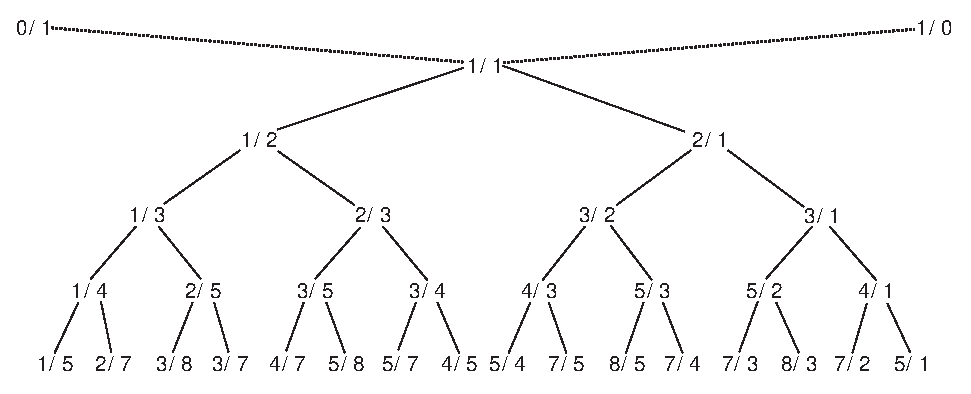
\includegraphics[width=4.6in]{c_cfr0/sbtdpt01.eps}
\caption{The Stern-Brocot Tree}
\label{fig:ccfr0:ssbt0:sdpt0:00}
\end{figure}

To construct the tree, one begins with the two fractions $\frac{0}{1}$
and $\frac{1}{0}$, and forms the mediant (see Definition 
\cfryzeroxrefhyphen{}\ref{def:cfry0:spfs:02})
of two adjacent fractions as many
times as desired to generate additional fractions.
Figure \ref{fig:ccfr0:ssbt0:sdpt0:00} illustrates the construction process.
Note in Figure \ref{fig:ccfr0:ssbt0:sdpt0:00} that the adjacent fractions
are always above and to the left and above and to the right of the fraction
being constructed, and that in the construction of the Stern-Brocot
tree, one of the adjacent fractions can be many levels upwards in the tree
from the fraction being constructed.  For example, in 
Figure \ref{fig:ccfr0:ssbt0:sdpt0:00}, when constructing the fraction 
4/5, the left adjacent fraction (3/4) is nearby in the figure, but 
the right adjacent fraction (1/1) is three levels up to the left and
one level up to the right.  Note when constructing the fraction 4/5 that
its right adjacent fraction is \emph{not} 4/3.

Note that it is also possible to maintain the Stern-Brocot tree as an
ordered list, rather than a tree, starting with the list
$\{0/1, 1/0\}$.  An additional element may be inserted
between any two existing elements in the list by forming their mediant,
and this process may be repeated indefinitely.  Note also that two 
elements $s_L$ and $s_R$ are Farey neighbors to any number $\alpha$
if $s_L < \alpha < s_R$ and the mediant of $s_L$ and $s_R$ has a
denominator larger than the order of the Farey series.  This gives a convenient
procedure for forming best rational approximations using only the Stern-Brocot
tree, as the following example shows.

\begin{vworkexamplestatement}
\label{ex:ccfr0:ssbt0:sdpt0:01}
Find the members of $F_{10}$ which enclose $\pi$.
\end{vworkexamplestatement}
\begin{vworkexampleparsection}{Solution}
By repeatedly calculating mediants, terms can be added to the list 
$\{\frac{0}{1}, \frac{1}{0} \}$ until $\pi$ is enclosed and it is not
possible to generate additional enclosing terms whose denominator does not
exceed 10.  This process is carried out below.

\begin{equation}
\left\{ {\frac{0}{1}, \frac{1}{0} } \right\}, 
\left\{ {\frac{0}{1}, \frac{1}{1}, \frac{1}{0} } \right\}, 
\left\{ {\frac{0}{1}, \frac{1}{1}, \frac{2}{1}, \frac{1}{0} } \right\}, 
\left\{ {\frac{0}{1}, \frac{1}{1}, \frac{2}{1}, \frac{3}{1}, \frac{1}{0} } \right\},
\end{equation}

\begin{equation}
\left\{ {\frac{0}{1}, \frac{1}{1}, \frac{2}{1}, \frac{3}{1}, 
         \frac{4}{1}, \frac{1}{0} } \right\}, 
\left\{ {\frac{0}{1}, \frac{1}{1}, \frac{2}{1}, \frac{3}{1}, \frac{7}{2},
         \frac{4}{1}, \frac{1}{0} } \right\}, 
\left\{ {\frac{0}{1}, \frac{1}{1}, \frac{2}{1}, \frac{3}{1}, \frac{10}{3}, \frac{7}{2},
         \frac{4}{1}, \frac{1}{0} } \right\}, 
\end{equation}

\begin{equation}
\left\{ {\frac{0}{1}, \frac{1}{1}, \frac{2}{1}, 
         \frac{3}{1}, \frac{13}{4}, \frac{10}{3}, \frac{7}{2},
         \frac{4}{1}, \frac{1}{0} } \right\}, 
\left\{ {\frac{0}{1}, \frac{1}{1}, \frac{2}{1}, 
         \frac{3}{1}, \frac{16}{5}, \frac{13}{4}, \frac{10}{3}, \frac{7}{2},
         \frac{4}{1}, \frac{1}{0} } \right\}, 
\end{equation}

\begin{equation}
\left\{ {\frac{0}{1}, \frac{1}{1}, \frac{2}{1}, 
         \frac{3}{1}, \frac{19}{6}, \frac{16}{5}, \frac{13}{4}, \frac{10}{3}, \frac{7}{2},
         \frac{4}{1}, \frac{1}{0} } \right\}, 
\end{equation}

\begin{equation}
\left\{ {\frac{0}{1}, \frac{1}{1}, \frac{2}{1}, 
         \frac{3}{1}, \frac{22}{7}, \frac{19}{6}, 
		 \frac{16}{5}, \frac{13}{4}, \frac{10}{3}, \frac{7}{2},
         \frac{4}{1}, \frac{1}{0} } \right\}, 
\end{equation}

\begin{equation}
\left\{ {\frac{0}{1}, \frac{1}{1}, \frac{2}{1}, 
         \frac{3}{1}, \frac{25}{8}, \frac{22}{7}, \frac{19}{6}, 
		 \frac{16}{5}, \frac{13}{4}, \frac{10}{3}, \frac{7}{2},
         \frac{4}{1}, \frac{1}{0} } \right\}. 
\end{equation}

Note that 25/8 and 22/7 are the left and right neighbors to
$\pi$ in $F_{10}$, since $25/8 < \pi < 22/7$, and since the 
mediant of 25/8 and 22/7 (49/15) has a denominator which is
too large for the Farey series being considered.

Note also that the construction process above could be 
trivially amended to treat the case of a constrained numerator 
rather than a constrained denominator.
\end{vworkexampleparsection}
\vworkexamplefooter{}

The Stern-Brocot tree has many remarkable properties (especially in view of the 
simplicity of its construction).  We mention the following properties
without proof.

\begin{itemize}
\item Each rational number in the tree is irreducible.

\item Each rational number appears in the tree only once.

\item Every positive rational number appears in the tree (i.e. there are no rational
      numbers absent).
\end{itemize}

A more detailed discussion of the Stern-Brocot tree and proof of its
properties is provided
in \cite{bibref:b:concretemathematics}, pp. 116-123.

%%%%%%%%%%%%%%%%%%%%%%%%%%%%%%%%%%%%%%%%%%%%%%%%%%%%%%%%%%%%%%%%%%%%%%%%%%%%%
%%%%%%%%%%%%%%%%%%%%%%%%%%%%%%%%%%%%%%%%%%%%%%%%%%%%%%%%%%%%%%%%%%%%%%%%%%%%%
%%%%%%%%%%%%%%%%%%%%%%%%%%%%%%%%%%%%%%%%%%%%%%%%%%%%%%%%%%%%%%%%%%%%%%%%%%%%%
\subsection{The Correspondence Between The Stern-Brocot Tree And The
            Apparatus Of Continued Fractions}
%Section tag:  DPT0
\label{ccfr0:ssbt0:sdpt1}

The Stern-Brocot tree, on examination, bears a clear resemblence to
the apparatus of continued fractions.  For example, in examining
Figure \ref{fig:ccfr0:ssbt0:sdpt0:00} and following leftmost branches in 
the tree, the rational numbers 1/2, 1/3, 1/4, and 1/5 correspond respectively
to the continued fractions [0;2], [0;3], [0;4], and [0;5].  Similarly,
following 
the right branches down from 1/2 yields, in order, [0;1,2], [0;1,3], and 
[0;1,4].  Clearly, a relationship between the Stern-Brocot tree and the
apparatus of continued fractions may exist.

Suspicions of a simple relationship may also arise by noting that the 
way in which the Stern-Brocot tree is constructed when only left branches
or only right branches are pursued is of the same form as the rule for
the formation of continued fraction convergents (Eqns. 
\ref{eq:thm:ccfr0:scnv0:canonicalconvergentconstruction:01}
and \ref{eq:thm:ccfr0:scnv0:canonicalconvergentconstruction:02}).  For example,
the $n$th successor to the right of 1/3 has the form

\begin{equation}
\label{eq:ccfr0:ssbt0:sdpt1:01}
\frac{n + 1}{2n+3},
\end{equation}

\noindent{}which is suspiciously similar to 
(\ref{eq:thm:ccfr0:scnv0:canonicalconvergentconstruction:01}) and 
(\ref{eq:thm:ccfr0:scnv0:canonicalconvergentconstruction:02}).

There is, in fact, an intimate relationship between the Stern-Brocot
tree and the apparatus of continued fractions.  We present 
this relationship as
Lemma \ref{lem:ccfr0:ssbt0:sdpt1:sbtcfcorrespondence}, 
below.

\begin{vworklemmastatement}
\label{lem:ccfr0:ssbt0:sdpt1:sbtcfcorrespondence}
Let $R^{z_0}L^{z_1} \ldots{} L^{z_{j-2}} R^{z_{j-1}} L^{z_{j}}$ 
or $R^{z_0}L^{z_1} \ldots{} R^{z_{j-2}} L^{z_{j-1}} R^{z_{j}}$
(depending on whether the final leg of the path is towards the
left or towards the right, respectively) be the path in the
Stern-Brocot tree from the fraction 1/1 to the fraction $a/b$, where
$L^N$ denotes traveling downward and to the left in the tree
$N$ nodes, and $R^N$ denotes traveling downward and to the right
in the tree $N$ nodes.  Then the continued fraction representation
of $a/b$ is $[z_0; z_1, \ldots{}, z_{j-2}, z_{j-1}, z_j + 1]$.
\end{vworklemmastatement}
\begin{vworklemmaproof}
The proof is inductive.  First note that the constraints of the path
require that $z_0 \geq 0$, and that $z_k \geq 1$, $k > 0$.  In other
words, only the first rightward leg of the path can have zero steps.

If the path is $R^{z_0}$, $z_0 = 0$, then the lemma predicts that the continued fraction
representation will be $[z_0 + 1]$ = $[1]$, which is the correct continued
fraction representation of the fraction 1/1.  Note that the rational number
1/1 has no ancestor in the tree.

If the path is $R^{z_0}$, $z_0 \neq 0$, then the lemma predicts that the
continued fraction representation will be $[z_0 + 1]$, which is correct
on inspection since the most rightward path in the Stern-Brocot tree
traverses the non-negative integers.  Note that the immediate ancestor of
the fraction $[z_0 + 1]$ is $[z_0]$.

If the path is $R^{z_0}, L^{z_1}$, $z_0 = 0$, then the
fraction $a/b$ will be the weighted mediant of
1/1 and 0/1,

\begin{equation}
\label{eq:ccfr0:ssbt0:sdpt1:02}
\frac{1}{z_1 + 1}
=
[0; z_1 + 1],
\end{equation}

\noindent{}which argrees with the lemma.  Note that the 
immediate ancestor ancestor of $[0; z_1 + 1]$ in the
tree is $[0; z_1]$. 

If the path is $R^{z_0}, L^{z_1}$, $z_0 \neq 0$, then the
fraction $a/b$ will be the weighted mediant of
$(z_0 + 1)/1$ and $z_0/1$, i.e.

\begin{equation}
\label{eq:ccfr0:ssbt0:sdpt1:03}
\frac{(z_0 + 1) + (z_0 z_1)}{(1) + (z_1)}
= z_0 + \frac{1}{z_1 + 1}
= [z_0; z_1 + 1],
\end{equation}

\noindent{}which is consistent with the lemma.  Note also that
the immediate ancestor of the rational number specified by
(\ref{eq:ccfr0:ssbt0:sdpt1:03}) is

\begin{equation}
\label{eq:ccfr0:ssbt0:sdpt1:03b}
\frac{(z_0 + 1) + z_0 (z_1 - 1)}{(1) + (z_1 - 1)}
= z_0 + \frac{1}{z_1}
= [z_0; z_1].
\end{equation}

The cases with two or fewer path components have been
proved above.  It remains to prove all cases with three
or more path components.

Let $s_k = p_k/q_k$ denote the $k$th-ordered convergent
of the continued fraction $[z_0; z_1, \ldots{}, z_{j-1}, z_j]$
(note that the final partial quotient is \emph{not} adjusted upwards by one).
For $k \geq 2$, we can establish a relationship between
$[z_0; z_1, \ldots{}, z_{k-1}, z_k]$
and
$[z_0; z_1, \ldots{}, z_{k-1}, z_k + 1]$ 
as follows:

\begin{equation}
\label{eq:ccfr0:ssbt0:sdpt1:04}
[z_0; z_1, z_2, \ldots{}, z_{k-2}, z_{k-1}, z_k + 1]
=
\frac{(z_k + 1)p_{k-1} + p_{k-2}}{(z_k + 1)q_{k-1} + q_{k-2}}
=
\frac{p_k + p_{k-1}}{q_k + q_{k-1}}.
\end{equation}

If we agree for convenience, as was mentioned in
Section \ref{ccfr0:scnf0}, that we will define $s_{-1} = p_{-1}/q_{-1} = 1/0$, 
then (\ref{eq:ccfr0:ssbt0:sdpt1:04}) holds for $k \geq 1$.

\textbf{(Inductive Step):} Assume that the lemma holds
up through $k-1$.  For a path in the Stern-Brocot tree
$R^{z_0}L^{z_1} \ldots{} L^{z_{k-2}} R^{z_{k-1}} L^{z_{k}}$ 
or $R^{z_0}L^{z_1} \ldots{} R^{z_{k-2}} L^{z_{k-1}} R^{z_{k}}$, 
$k \geq 2$, the ``reversal'' fraction above (i.e. the fraction where the path changes
directions) is

\begin{equation}
\label{eq:ccfr0:ssbt0:sdpt1:05}
[z_0; \ldots{}, z_{k-2}, z_{k-1} + 1] = 
\frac{p_{k-1} + p_{k-2}}{q_{k-1} + q_{k-2}}
\end{equation}

\noindent{}(this is established by the lemma on the path through $k-1$ and by
Eqn. \ref{eq:ccfr0:ssbt0:sdpt1:04}).

The immediate ancestor of the fraction specified in 
(\ref{eq:ccfr0:ssbt0:sdpt1:05}) is

\begin{equation}
\label{eq:ccfr0:ssbt0:sdpt1:06}
[z_0; \ldots{}, z_{k-2}, z_{k-1}] = 
\frac{z_{k-1}p_{k-2} + p_{k-3}}{z_{k-1}q_{k-2} + q_{k-3}} ,
\end{equation}

\noindent{}as was shown to hold in (\ref{eq:ccfr0:ssbt0:sdpt1:03b}) and
in the inductive step.

The rational number corresponding to the path
$R^{z_0}L^{z_1} \ldots{} L^{z_{k-2}} R^{z_{k-1}} L^{z_{k}}$ 
or $R^{z_0}L^{z_1} \ldots{} R^{z_{k-2}} L^{z_{k-1}} R^{z_{k}}$
is a weighted mediant of (\ref{eq:ccfr0:ssbt0:sdpt1:05}) 
and (\ref{eq:ccfr0:ssbt0:sdpt1:06}):

\begin{eqnarray}
\label{eq:ccfr0:ssbt0:sdpt1:07}
\hspace{-0.35in}
\frac{z_k(z_{k-1}p_{k-2} + p_{k-3}) + p_{k-1} + p_{k-2}}
     {z_k(z_{k-1}q_{k-2} + q_{k-3}) + q_{k-1} + q_{k-2}}
 & = &
\frac{(z_k + 1)p_{k-1} + p_{k-2}}{(z_k + 1)q_{k-1} + q_{k-2}} \\
\label{eq:ccfr0:ssbt0:sdpt1:08}
& = & \frac{p_k + p_{k-1}}{q_k + q_{k-1}} \\
& = & [z_0; z_1, \ldots{}, z_{k-1}, z_{k} + 1],
\end{eqnarray}

\noindent{}which establishes the main result of the lemma in the
inductive step.  Note also that the immediate ancestor of the
fraction specified in (\ref{eq:ccfr0:ssbt0:sdpt1:07}) is 
$[z_0; \ldots{}, z_{k-1}, z_{k}]$ (which is necessary for 
the inductive step).  This proves the lemma.
\end{vworklemmaproof}
\begin{vworklemmaparsection}{Remarks}
This lemma provides a straightforward method to go from a
fraction's position in the Stern-Brocot tree to its continued
fraction representation, or vice-versa.

To go from a fraction's position in the Stern-Brocot tree to its
continued fraction representation:

\begin{itemize}
\item Starting with moves downward and to the right from the
      fraction 1/1 ($z_0$), observe the length of the alternating
      rightward and leftward node traversals required to reach
	  the desired fraction.

\item Adjust the final length upward by one.

\item These lengths in order are then the successive partial quotients
      of the fraction.
\end{itemize}

To go from the continued fraction representation of a fraction
to its position in the Stern-Brocot tree:

\begin{itemize}
\item Reduce the final partial quotient by one.

\item Use the partial quotients, in order, in an alternating fashion,
      to go rightward and downward
      and leftward and downward in the Stern-Brocot tree.  The fraction
	  reached on the final leg will be the fraction of interest.
\end{itemize}
\end{vworklemmaparsection}
\vworklemmafooter{}

It is clear from the lemma above that the Stern-Brocot tree and the 
apparatus of continued fractions are intimately related.  Specifically,
the Stern-Brocot tree provides a model for the formation and arrangement
of rational numbers, but the apparatus of continued fractions provides
a much more efficient way to navigate the Stern-Brocot tree and to find
best rational approximations.

%%%%%%%%%%%%%%%%%%%%%%%%%%%%%%%%%%%%%%%%%%%%%%%%%%%%%%%%%%%%%%%%%%%%%%%%%%%%%
%%%%%%%%%%%%%%%%%%%%%%%%%%%%%%%%%%%%%%%%%%%%%%%%%%%%%%%%%%%%%%%%%%%%%%%%%%%%%
%%%%%%%%%%%%%%%%%%%%%%%%%%%%%%%%%%%%%%%%%%%%%%%%%%%%%%%%%%%%%%%%%%%%%%%%%%%%%
\subsection{Using The Stern-Brocot Tree To Find Best Rational Approximations}
%Section tag:  USB0
\label{ccfr0:ssbt0:susb0}

It is clear from Example \ref{ex:ccfr0:ssbt0:sdpt0:01} that the Stern-Brocot
tree can be used to find best rational approximations in the Farey series
of any order, simply by forming mediants until the number of interest
is enclosed.  It is also clear that an algorithm of repeatedly forming
mediants in order to find a best rational approximation in
$F_{k_{MAX}, \overline{h_{MAX}}}$ can be devised.

However, the sole drawback of such a procedure is that building the Stern-Brocot
tree from the top in order to find neighbors in $F_N$ is an
$O(N)$ procedure, which renders it unsuitable for use with large
$N$.  For this reason, the continued fraction algorithms presented
earlier in the chapter, which are $O(log \; N)$ (due to the 
guaranteed minimum exponential rate of increase of convergent
denominators, Theorem \ref{thm:ccfr0:scnv0:minimumrateofconvergentdenominatorincrease}),
are the only practical algorithms.


%%%%%%%%%%%%%%%%%%%%%%%%%%%%%%%%%%%%%%%%%%%%%%%%%%%%%%%%%%%%%%%%%%%%%%%%%%%%%
%%%%%%%%%%%%%%%%%%%%%%%%%%%%%%%%%%%%%%%%%%%%%%%%%%%%%%%%%%%%%%%%%%%%%%%%%%%%%
%%%%%%%%%%%%%%%%%%%%%%%%%%%%%%%%%%%%%%%%%%%%%%%%%%%%%%%%%%%%%%%%%%%%%%%%%%%%%
\section{Practical Techniques}
%Section tag:  PTQ0

Although this chapter has presented rather theoretical results and techniques
from number theory, our emphasis is on practical applications (which is why
we've concentrated on finding Farey neighbors of \emph{rational} numbers).
Practicing engineers would be more likely to use the digits from a calculator
as the starting point to obtain a rational approximation than to use 
a symbolic irrational constant, such as $\pi$.

In this section, we present \emph{practical} techniques---those most likely
to be used in practice by microcontroller software developers.



%%%%%%%%%%%%%%%%%%%%%%%%%%%%%%%%%%%%%%%%%%%%%%%%%%%%%%%%%%%%%%%%%%%%%%%%%%%%%
%%%%%%%%%%%%%%%%%%%%%%%%%%%%%%%%%%%%%%%%%%%%%%%%%%%%%%%%%%%%%%%%%%%%%%%%%%%%%
%%%%%%%%%%%%%%%%%%%%%%%%%%%%%%%%%%%%%%%%%%%%%%%%%%%%%%%%%%%%%%%%%%%%%%%%%%%%%
\subsection{Practical Aspects Of Beginning With A Rational Approximation}
%Subsection tag:  PAS0
\label{ccfr0:sptq0:sspas0}

In practical applications, one often begins with a rational approximation 
to a irrational number.  
For example, one might use 3.14159265359 (from
a calculator) as the value of $\pi$ for the application of 
Algorithm \ref{alg:ccfr0:scrn0:akgenalg}.  This naturally raises the
question of how accurate the rational approximation used
as a starting point must be to avoid identifying the wrong 
rational numbers as Farey neighbors.  We illustrate the possibility
of identifying the wrong rational number with an example.

\begin{vworkexamplestatement}
\label{ex:ccfr0:sptq0:01}
Find the members of $F_{255}$ which enclose $\pi$, using 
3.1416 as the value of $\pi$.
\end{vworkexamplestatement}
\begin{vworkexampleparsection}{[Erroneous] Solution And Remarks}
It can be shown using the methods presented earlier that
the members of $F_{255}$ which enclose 3.1416 are
355/113 and 732/333, i.e.

\begin{equation}
\frac{355}{113} < 3.1416 < \frac{732}{333} .
\end{equation}

However, in fact, 688/219 and 355/113 are the actual enclosing
neighbors of $\pi$ in $F_{255}$:

\begin{equation}
\frac{688}{219} < \pi < \frac{355}{113} < 3.1416 < \frac{732}{333} .
\end{equation}

Thus by using an imprecise approximation of $\pi$, we have incorrectly
identified the neighbors to $\pi$ in $F_{255}$.
\end{vworkexampleparsection}
\vworkexamplefooter{}

How do we avoid incorrectly identifying the rational
numbers which enclose an irrational number when a
rational approximation of the irrational number is
used as the starting point for the selection algorithm?
There are three practical approaches to the problem.

Observe that when we know
the first several decimal digits of an irrational number,
the actual value of the irrational number is confined
to an interval.  For example, if a calculator displays
``3.1416'' as the value of $\pi$, we might safely
assume that $3.14155 \leq \pi \leq 3.14165$, if the
digits that the calculator displays were 
obtained by rounding.  

As a first approach to dealing with a rational approximation
to an irrational number,
we might simply determine the
Farey neighbors of both endpoints of the interval of
uncertainty.  For example, if
314,155/100,000 and 314,165/100,000 have the same 
Farey neighbors in a Farey series of interest (which we can
easily determine using the algorithms presented earlier
in this chapter), we could
correctly deduce that these Farey neighbors are the
Farey neighbors of $\pi$.  On the other hand,
if 314,155/100,000 and 314,165/100,000 have different
enclosing Farey neighbors, then there are Farey 
terms in the interval [3.14155, 3.14165],
and more information about $\pi$
would be required to determine its true Farey neighbors.

A second approach to this same problem would be to devise an
algorithm to process
the endpoints of the interval of uncertainty simultaneously and note
when their partial quotients diverge.  

A third approach, which is 
perhaps the most direct, is to apply 
Algorithm \cfryzeroxrefhyphen{}\ref{alg:cfmindenominator} to determine
the rational number with the minimum denominator in the interval of uncertainty.
We would thus know that we have enough information to determine uniquely the
enclosing rational numbers in any Farey series up to one less than this 
minimum denominator.

\begin{vworkexamplestatement}
\label{ex:ccfr0:sptq0:02}
Assume that 3.142 is the only value for $\pi$ available.  What is the maximum
order of the Farey series where the enclosing rational numbers to $\pi$ can
be unambiguously determined?
\end{vworkexamplestatement}
\begin{vworkexampleparsection}{Solution}
Assume that the constant ``3.142'' was obtained by rounding of digits, rather than
by truncation of digits:  thus $3.1415 \leq \pi \leq 3.1425$.  Applying
Algorithm \cfryzeroxrefhyphen{}\ref{alg:cfmindenominator} yields 333/106
as the rational number with the smallest denominator in the interval
[3.1415, 3.1425].  Thus, no rational number with a smaller denominator exists
in the interval, and the enclosing rational numbers of $\pi$ in the Farey series of
up to order 105 can be determined with the limited information available.
\end{vworkexampleparsection}
\vworkexamplefooter{}


%%%%%%%%%%%%%%%%%%%%%%%%%%%%%%%%%%%%%%%%%%%%%%%%%%%%%%%%%%%%%%%%%%%%%%%%%%%%%
%%%%%%%%%%%%%%%%%%%%%%%%%%%%%%%%%%%%%%%%%%%%%%%%%%%%%%%%%%%%%%%%%%%%%%%%%%%%%
%%%%%%%%%%%%%%%%%%%%%%%%%%%%%%%%%%%%%%%%%%%%%%%%%%%%%%%%%%%%%%%%%%%%%%%%%%%%%
\subsection{Obtaining Irrational Numbers To High Precision}
%Subsection tag:  OIN0
\label{ccfr0:sptq0:ssoin0}

It may happen in practice that one desires more information about an
irrational number than can be easily obtained.  As a practical example,
a typical scientific calculator treats $\pi$ as 3.14159265359, implying that 
$3.141592653585 \leq \pi \leq 3.141592653595$.  Application of 
Algorithm \cfryzeroxrefhyphen{}\ref{alg:cfmindenominator} to this
interval yields 1,146,408/364,913 as the rational number with the
smallest denominator in this interval:  implying that we cannot determine the 
enclosing rational approximations to $\pi$ even in $F_{2^{32}-1}$ using
the information most readily available.  How do we obtain more digits of $\pi$?
And even if we can obtain more digits of $\pi$, how do we manipulate rational
numbers with such large integer components?  (We discuss the problem of obtaining
more digits below, but discuss manipulation in Section \ref{ccfr0:sptq0:smhp0}.)

There are two approaches to determining $\pi$ or other numbers to
high precision.

\begin{enumerate}

\item Locate information about the number on the Web or in a reference
      book.  (Note that decimal digits of the number, partial quotients
	  of the number, or convergents of the number can all be used; and it
	  is typical for all of these to be somewhere on the Web.  However,
	  convergents are the most useful form for obtaining best rational
	  approximations.)

\item Use commercial symbolic manipulation software (\index{Mathematica@\emph{Mathematica}}\emph{Mathematica}
      \cite{bibref:s:wolframmathematica}, 
      for example) to
      obtain the number of interest to arbitrary 
      precison.\footnote{\label{footnote:ccfr0:sptq0:ssoin0:mathematicaexpensive}\emph{Mathematica}
      \cite{bibref:s:wolframmathematica} is quite expensive (version 4.1 
      for Windows, as of March 2001, is \$1,495), 
      and something that a microcontroller software developer
      would very rarely use, so we assume that most microcontroller software
      developers would search for a less expensive solution.}

\end{enumerate}

%%%%%%%%%%%%%%%%%%%%%%%%%%%%%%%%%%%%%%%%%%%%%%%%%%%%%%%%%%%%%%%%%%%%%%%%%%%%%
%%%%%%%%%%%%%%%%%%%%%%%%%%%%%%%%%%%%%%%%%%%%%%%%%%%%%%%%%%%%%%%%%%%%%%%%%%%%%
%%%%%%%%%%%%%%%%%%%%%%%%%%%%%%%%%%%%%%%%%%%%%%%%%%%%%%%%%%%%%%%%%%%%%%%%%%%%%
\subsection{Manipulating High-Precision Rational Numbers}
%Subsection tag:  MHP0
\label{ccfr0:sptq0:smhp0}

Assuming that one is able to determine a [rational or irrational] number
of interest to high-precision (either a large number of decimal digits or a rational
number with large integer components), how does
one manipulate rational numbers with large integer components?
In this section, we list software alternatives.

The first alternative we should mention is \emph{The Iju Tool Set}, distributed
with this book.  Starting with version 1.05, this tool set contains
a subset of the GNU MP Library \cite{bibref:s:gnumultipleprecisionarithmeticlibrary}, 
and will manipulate 
large integers and rational numbers with large integer components.  To provide
more flexibility for the user, this tool set is embedded as extensions to
the Tcl scripting language; so that any of the functionality provided can be
used either interactively or from within a Tcl script.

\begin{figure}
\centering
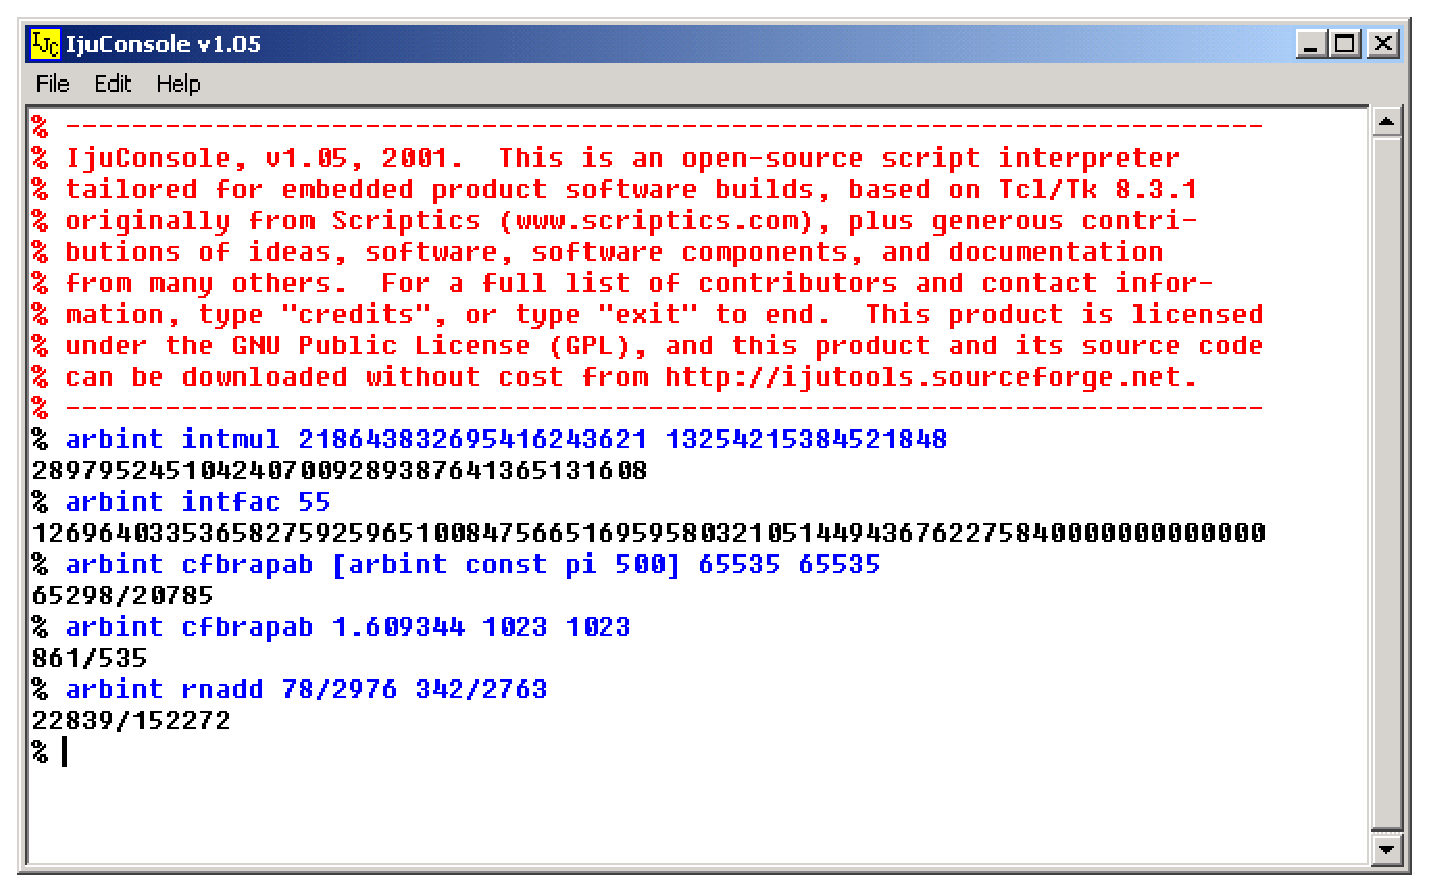
\includegraphics[width=4.6in]{c_cfr0/ijt_ss01.eps}
\caption{Large Integer Arithmetic And Best Rational Approximations Using \emph{IjuConsole}
         From \emph{The Iju Tool Set}}
\label{fig:ccfr0:sptq0:smhp0:00}
\end{figure}

Figure \ref{fig:ccfr0:sptq0:smhp0:00} shows a screen snapshot\footnote{By
the way, \emph{IjuConsole} will handle \emph{much} larger integers, but 
small examples were used so that all of the information would fit
in a single screen snapshot.} of
\emph{IjuConsole} (the \emph{Wish}-like Tcl
interpreter from \emph{The Iju Tool Set}) being used interactively
to provide the answers to several questions involving large integers and
rational numbers with large integer components.  The first command
shown,\\

\texttt{arbint intmul 218643832695416243621 13254215384521848},\\

\noindent{}illustrates integer multiplication.  The second command shown,\\

\texttt{arbint intfac 55},\\ 

\noindent{}illustrates calculating the factorial of
55.  The third command shown, \\

\texttt{arbint cfbrapab [arbint const pi 500] 65535 65535},\\

\noindent{}illustrates calculating the best rational approximation to 
$\pi$ with numerator and denominator not exceeding 
65,535, and using the first 500 digits of $\pi$ as
the value of $\pi$.  The fourth command shown,\\

\texttt{arbint cfbrapab 1.609344 1023 1023},\\

\noindent{}illustrates finding the best rational approximation to 
the conversion factor from MPH to KPH with numerator and denominator
not exceeding 1,023.  The last command shown,\\

\texttt{arbint rnadd 78/2976 342/2763},\\

\noindent{}illustrates the addition of
two rational numbers.

Many other potential solutions for dealing with large
integers have been submitted by newsgroup
posters, and are listed below.  (Please note that these alternatives haven't actually been
tried, and we can't say whether they are viable.)

\begin{enumerate}

\item \index{Mathematica@\emph{Mathematica}}\emph{Mathematica} 
      \cite{bibref:s:wolframmathematica} (by Wolfram Research) will easily operate on large integers and 
      rational numbers with large integer components  (see
      Footnote \ref{footnote:ccfr0:sptq0:ssoin0:mathematicaexpensive}).
      (Suggested by \index{Lutus, Paul} Paul Lutus \cite{bibref:i:paullutus} and
      \index{Taylor, Don} Don Taylor \cite{bibref:i:dontaylor}.)

\item \index{GNU!Multiple Precision Arithmetic Library (GMP)}The 
      \emph{GNU Multiple Precision Arithmetic 
      Library (GMP)} \cite{bibref:s:gnumultipleprecisionarithmeticlibrary}.
      This library, which is free and on the Web, can be linked into
      `C' and `C++' programs, and allows fast integer calculations of
      any size that do not exceed the memory available in the computer.
      This library could be used to quickly construct a program to 
      process rational numbers with very large integer components.

\item \index{UBASIC@\emph{UBASIC}}\emph{UBASIC} \cite{bibref:s:ubasic} 
      (\index{Kida, Yuji}by Yuji Kida \cite{bibref:i:yujikida})
      is an extended-precision version of the BASIC
      language which will handle integers up to 2,600 digits and
      exact rational arithmetic. (Suggested by \index{Schorn, Richard} Richard Schorn 
      \cite{bibref:i:richardschorn}.)

\item \index{Derive 5@\emph{Derive 5}}\emph{Derive 5} \cite{bibref:s:derive5} (by Texas Instruments).
      The exact capabilities of this software are not known, but the Web page indicates
      it can perform exact rational arithmetic.  (Suggested by \index{Schorn, Richard} Richard Schorn 
      \cite{bibref:i:richardschorn} and \index{Taylor, Don} Don Taylor \cite{bibref:i:dontaylor}.)

\item \index{Maple@\emph{Maple}}\emph{Maple} \cite{bibref:s:maple} (by Waterloo
      Maple, Inc.).  The exact capabilities of this software are not known.
      (Suggested by 
      \index{Lutus, Paul} Paul Lutus \cite{bibref:i:paullutus} and
      \index{Taylor, Don} Don Taylor \cite{bibref:i:dontaylor}.)

\item \index{MuPAD@\emph{MuPAD}}\emph{MuPAD} \cite{bibref:s:mupad} (from
      the University Of Paderborn, Germany).  The capabilities of this
      software are not known.  (Suggested by \index{Schorn, Richard} Richard Schorn 
      \cite{bibref:i:richardschorn}.)

\end{enumerate}

%http://www.csc.fi/math_topics/Mail/FAQ/msg00015.html

In addition to the large integer resources above, a 
much longer list of resources is maintained
at the URL

\begin{quote}
\texttt{http://www.csc.fi/math\_topics/Mail/FAQ/msg00015.html},
\end{quote}

\noindent{}and is reproduced below.  Because this URL was apparently last updated
in 1994, it is not known which of the resources listed are still
available.

\begin{quote}
\begin{scriptsize}
\begin{verbatim}
--------------------------------------------------------------------------------
Subject: List of Arbitrary Precision C packages 
From: mrr@scss3.cl.msu.edu (Mark Riordan) 
Date: 27 Jan 1994 16:06:01 GMT 
Newsgroups: sci.math 
--------------------------------------------------------------------------------
This is the file BIGNUMS.TXT from ripem.msu.edu, last updated January 1994.

In response to Email requests, I have assembled this list of
large-integer arithmetic packages of which I have heard.
Most of these are C function libraries, available in source form.
A few also deal with floating point numbers.  

For your convenience, I have placed copies of
some of these on ripem.msu.edu (35.8.1.178).  They are
available for anonymous FTP in the directory "pub/bignum".
However, what I have may not be the most current version in all cases.

Here they are, in no particular order:

mp
    Multiple Precision package that comes with some Unixes
    
    Multiple precision package accessed via -lmp flag on your
    compiler.  Provides +, -, *, /, gcd, exponentiation,
    sqrt.  Comes with SunOS, NeXT Mach, BBN Mach 1000, 
    and probably a few others.  See "man 3 mp".  
    Object code only, of course.

PARI
    Henri Cohen, et al., Universite Bordeaux I, Paris, FRANCE
    
    Multiple precision desk calculator and library routines.
    Contains optimized assembly code for Motorola 68020, 
    semi-optimized code for SPARC, and apparently rather slow
    generic C version.  Does both integers and reals.
    Does vectors and matrices as well as scalars.
    Contains a number of advanced functions, some of which I've
    never heard of.  ("Weber's function"?)
    Has a factorization function, primality test, & other related stuff.
    Plenty of TEX documentation.
    Public domain, but you can't distribute modified versions.
    Available via anonymous FTP from ftp.inria.fr:lang/ and 
    math.ucla.edu.  The ucla site has Mac, MSDOS, OS/2, and
    NeXT-specific versions there in addition to:
    Filename:  pari-1.37.tar.Z  (There are now more recent versions)
    
Arithmetic in Global Fields  (Arith)
    Kevin R. Coombes, David R. Grant
    
    Package of routines for arbitrary precision integers or
    polynomials over finite fields.  Includes basic +, -, *, /
    and a few others like gcd.  Source code in C.
    Distributed under the terms of the GNU public license.
    Includes man pages and TEX documentation.
    Filename:  arith.tar.Z

Arbitrary Precision Math Library
    Lloyd Zusman   Los Gatos, CA
    
    C package which supports basic +, -, *, /.  Provides for radix
    points (i.e., non-integers).  Not as polished as the others here.
    Posted to comp.sources.misc in October 1988.
    Filename:  apml.tar.Z
    
BigNum
    J. Vuillemin, INRIA, FRANCE, and others.
    Distributed by Digital Equipment Paris Research Lab (DECPRL)
    
    A "portable and efficient arbitrary-precision integer" package.
    C code, with generic C "kernel", plus assembly "kernels" for
    MC680x0, Intel i960, MIPS, NS32032, Pyramid, and of course VAX.
    This is probably one of the better-known packages of this type.
    Implements +, -, *, /, mod, plus logical operations OR, AND, XOR.
    Both signed and unsigned arithmetic available.
    Available via email from librarian@decprl.dec.com.
    You will receive 5 shell archives.  Give your postal address
    and you will also receive printed documentation from France.
    Package includes TEX documentation.
    Publicly available for non-commercial use.
    I removed this from my archive when I heard a rumor that PRL
    doesn't like others to distribute it.  However, BIGNUM *is*
    distributed as part of ecpp (see below).

Lenstra's LIP package
    Arjen Lenstra   Bellcore
    
    Portable unsigned integer package written entirely in C.
    Includes +, -, *, /, exponentiation, mod, primality testing,
    sqrt, random number generator, and a few others.  
    An earlier version of this package is the only of these packages
    I have actually used.  It works well and is very portable.  
    I haven't done any benchmarks against the others, but the code 
    looks clever & Lenstra is an accomplished number theorist.

    LIP replaces lenstra-3.1.c.  The package now includes encrypted
    source code; to obtain the decryption key, you must send a
    signed license agreement to Bellcore.  See the documentation.
    Filename:  lenstra-LIP-package.tar  This is a collection of
    all the files in flash.bellcore.com:/pub/lenstra

bmp  (Brent's Multiple Precision?)
    R. P. Brent

    1981 vintage FORTRAN code to do extended precision floating &
    fixed point arithmetic.  Includes most of the mathematical
    functions you'd find in a FORTRAN run-time library.
    This code is an ACM algorithm, number 524.
    To obtain, send a mail message to  netlib@ornl.gov
    containing the line "send mp.f from bmp" or better yet, perhaps
    just start with "help".

SPX
    Kannan Alagappan & Joseph Tardo, DEC
    
    This is a huge prototype public key authentication system
    based on RSA.  I mention it here because those who have heard
    of SPX have probably correctly guessed that it contains a large
    integer package and I want to inform you that the large integer
    package it contains is indeed DEC's BigNum from France.
    You can get a beta test copy of SPX from crl.dec.com (192.58.206.2). 
    Use it only for testing, as it "may" expire on a certain date.
    (I don't know whether this has expired yet.)

amp  (Antti's Multiple Precision?)
    Antti Louko   alo@kampi.hut.fi

    Multiple precision integer package in C.  Includes +, -, *, /, %,
    pow, mod, 1/x mod y, random, sqrt, gcd.  Available for non-commercial
    use.  The package includes "share-secret", a public key system based
    on the Diffie-Hellman algorithm.
    This is normally part of the well-known "des-dist.tar.Z",
    but I have removed the DES part to avoid having to deal with 
    cryptographic export laws, and have named the result:
    Filename:  amp.tar.Z

gennum  
    Per Bothner   U of Wisconsin-Madison

    C++ routines and classes to do generic arithmetic, both
    integer and rational.  Part of the "Q" programming system.
    Distributed under the terms of the GNU public license.
    Obtained from cygnus.com.
    Filename: gennum.tar.Z

MIRACL
    (Shamus Software, Dublin, Ireland)

    Integer and fractional multiple precision package.
    MIRACL is a portable C library. Full C/C++ source code included 
    (In-line assembly support for 80x86). Number theoretic primitives
    needed to support PK Cryptography are supplied.   
    C++ classes for Multiprecision Integers, Modular arithmetic, and 
    Chinese Remainder Thereom. Implementation in C/C++ of all modern 
    methods of Integer Factorisation, viz Brent-pollard, p-1, p+1, 
    Elliptic Curve, MPQS.  Includes TEX manual and some DOS .EXEs.
    Not public domain, but free for academic and non-commercial use.
    Obtained from ftp.compapp.dcu.ie.
    Filename:  /pub/crypt/other/miracl-3.23.zip and miracl.tar.Z (older)

precision
    Dave Barrett  barrettd@tigger.colorado.edu

    Multiple precision integer package in C with +,-,*,/, sqrt, rand,
    mod, pow, log.  Simple vector support.  Does dynamic allocation of memory.
    Free as long as you don't sell it or any program that uses it.
    Filename:  precision.tar.Z

UBASIC
    Prof. Yuji Kida, Rikkyo University, Nishi-Ikebukuro 3, Tokyo 171, Japan
    kida@rkmath.rikkyo.ac.jp

    Multiple-precision version of the BASIC programming language,
    for MS-DOS.  Includes floating point.  Said (by Keith Briggs)
    to be pretty fast.  Object only, I think.  ervin@morekypr.bitnet
    says:  "This is the best package that I know of for
    fast arithmetic.  Has a version optimized for 386 machines.  Includes
    routines to do MPQS, the fastest currently known general factoring
    algorithm.  An additional file is at both sites to allow MPQS to use
    hard drives so that it can factor up to 80 digits.  Many number
    theoretical functions are included in UBASIC.  It allows over 2500
    digits of precision."
    Available via anonymous FTP from shape.mps.ohio-state.edu,
    or simtel20.army.mil, or wuarchive.wustl.edu.

calc_v22
    Unknown

    MS-DOS C-like language that allows "infinite" precision.
    Nice intrinsic functions.  ervin@morekypr.bitnet reports problems
    when changing precision on the fly.
    See simtel20 or wuarchive.

briggs_arith
    Keith Briggs (kbriggs@maths.adelaide.edu.au)

    Turbo Pascal 5 source for routines that do multiple-precision
    +, -, *, /, sqrt, gcd, factoring, rand for integers; also includes
    +, -, *, / and rand for rational numbers.
    Filename:  briggs_arith.pas

Institute fur Experimentelle Mathematik
    Dr Gerhard Schneider (?)

    Fast C multiple-precision subroutine library.
    I don't know anything about it; sl25@ely.cl.cam.ac.uk says
    to contact MAT420@DE0HRZ1A.BITNET for more info.
    Postal Address:
    Institute fur Experimentelle Mathematik
    EllernStr 29
    D4300 Essen-12    GERMANY

LongInt
    Markus Mueller (mueller@komsys.tik.ethz.ch)

    "Multi precision arithmetic written in MODULA-2, with the most time critical
    parts written in Assembler. Includes basic arithmetics (+, -, *, /, %) as
    well as arithmetics MODULO a number. An additional module provides a
    collection of procedures for primality testing, gcd, multiplicative
    inverse and more. The package is part of a Privacy Enhanced Mail (PEM)
    package which includes a PEM mailer, RSA key generator and Certificate
    generation tools."

    Source is in Modula-2, C, and assembler for Sun 3.  LongInt has
    also been ported to MS-DOS under Logitech Modula-2 and Turbo
    Assembler.  Availability:  free for university use (research and
    education); otherwise, a source license is required.  To obtain,
    write or email to:

        Markus Mueller
        Bertastrasse 7
        CH-8953 Dietikon
        Switzerland
        email:  mueller@komsys.tik.ethz.ch

bignum-1.2
    Henrik.Johansson@Nexus.Comm.SE

    Bignum package written in portable C.  Will in the future
    conform to the Common Lisp functions that handles integers.
    Currently includes +, -, *, /, exponentiation, "exptmod",
    comparison, random numbers, and gcd.
    Filename: bignum-1.2

ACM algorithm 567
    D.W. LOZIER and J.M. SMITH

    FORTRAN subroutines to do extended-precision floating point
    and normalized Legendre polynomials.
    ACM TRANSACTIONS ON MATHEMATICAL SOFTWARE 7,1 (MARCH, 1981)
    Obtained from research.att.com:netlib/toms/567.Z
    Filename: acm-algorithm-567-floating-point.fortran.Z

range
    O. Aberth and M. J. Schaefer

    C++ package to do extended-precision floating point arithmetic
    with programmer-defined precision.  Uses decimal representations
    internally.  Contains basic +, -, *, /, relational operators,
    ++, and a few functions like sin, cos, sqrt, log.  Documentation
    a trifle confusing.
    Obtained from math.tamu.edu:pub/range/range.tar.Z
    Filename: range.tar.Z

bsint
    Author unknown.

    Pre-alpha release of C++ big integer package.  
    Implements basic math operators, exponentiation, and modular 
    exponentiation.  Very skimpy documentation.
    See milton.u.washington.edu:/pub/user-supported/tzs/bsint.tar.Z

GNU Multiple Precision (GMP)
    GNU (Free Software Foundation) multiple precision package.
    I haven't looked at it yet.  This is current as of April 1992,
    but there may be a more recent version by the time you read 
    this.  This package is very widely available on FTP sites.
    Filename: gmp-1.3.2.tar.Z

libg++ - GNU's C++ class library
    Free Software Foundation

    Includes Integer and Rational classes.  Integer provides
    the usual C++ operators, plus exponentiation, gcd, lcm.
    Limited functionality, but documentation is better than most.
    Look for libg++-2.4.tar.gz on an FTP server near you.

Elliptic Curve Primality Proving 
    Francois Morain, France.

    Large package to prove the primality of any prime.
    Includes Inria's BIGNUM package. 
    Obtained from ftp.inria.fr (128.93.1.26).
    Filename: ecpp.V3.4.1.tar.Z

PGP (Pretty Good Privacy)
    Philip Zimmermann   prz@sage.cgd.ucar.EDU

    Crypto package that includes bignum routines in C.
    Assembly implementations available for several processors;
    said to be quite fast for numbers around 1000 bits in size.
    The crypto package violates RSA patents, but the bignum routines
    can be used without fear of legal repercussions.

Bell's Arbitrary Precision Calculator
    David I. Bell, Australia  (dbell@pdact.pd.necisa.oz.au)

    Arbitrary-precision calculator with good online help, C-like
    language, many builtin functions, support for integers,
    rational numbers (they work like floating point), complex numbers,
    matrices, strings, lists, files, "objects".  Includes 
    gcd, primality testing, even trig functions.  Recommended.
    (Large package, though.)  Obtained from comp.sources.unix.
    Filename: calc-1.24.7.tar.Z

Calc for GNU Emacs
    Dave Gillespie  (daveg@synaptics.com)
   
    Advanced calculator written in Emacs Lisp.  Includes arbitrary
    precision integers and floating point, bitwise operations,
    log and trig functions, financial functions, number theoretic
    functions including prime factorization, symbolic calculus,
    and an interface to GNUPLOT.
    Filename:  calc-2.02a.tar.Z

MPFUN: A Multiple Precision Floating Point Computation Package
    David H. Bailey   (dbailey@nas.nasa.gov)

    Package of Fortran subroutines to perform multiprecision
    floating point arithmetic.  Also includes a program that
    can automatically convert ordinary Fortran-77 code into code
    that calls the MPFUN routines.  
    Keith Briggs says: "It's a masterpiece, and the state of the art 
    as far as Fortran goes."
    Documentation in TeX format.  Unrestricted distribution
    allowed at no cost.
    Filenames: mpfun_fortran.tar.Z & mpfun_tex_papers.tar.Z

MPQS
    Mark S. Manasse  (msm@src.dec.com)  and Arjen Lenstra

    C program to factor numbers on a distributed network of
    heterogeneous machines.  June 1993 version.
    Filename:  mpqs-distributed-factoring.shar

GNU bc
   Author: Philip A. Nelson (phil@cs.wwu.edu)
   GNU bc is an interactive algebraic language with arbitrary precision.
   GNU bc is almost the same as bc & dc in some Unixes.
   Filename: bc-1.02.tar.z  (for example, in GNU prep.ai.mit.edu:pub/gnu/)

bc & dc
  bc is an interactive processor for an arbitrary precision arithmetic
  language or just compiler/preprocessor for dc calculator with arbitrary
  precision; they comes with some Unixes.

Built-in support in other languages
    Various

    Multiple precision arithmetic is available in a number of 
    programming languages, such as Lisp and ABC (cf. mcsun.eu.net).
    Version 8 of the programming language Icon (Griswold's successor
    to SNOBOL4 available from cs.arizona.edu) has large integers.
    Perl (by Larry Wall, available from devvax.jpl.nasa.gov)
    includes source, in Perl, for such a package, but it's probably
    not suitable for serious use.
    For some of these, source code may be available.  This list is
    long enough, so I'm not going to pursue it aggressively.

Thanks to Keith Briggs and several others who contributed to this list.

See also other sites, such as nic.funet.fi:pub/sci/math/multiplePrecision/.

Mark Riordan   mrr@ripem.msu.edu
--------------------------------------------------------------------------------
\end{verbatim}
\end{scriptsize}
\end{quote}



%%%%%%%%%%%%%%%%%%%%%%%%%%%%%%%%%%%%%%%%%%%%%%%%%%%%%%%%%%%%%%%%%%%%%%%%%%%%%
%%%%%%%%%%%%%%%%%%%%%%%%%%%%%%%%%%%%%%%%%%%%%%%%%%%%%%%%%%%%%%%%%%%%%%%%%%%%%
%%%%%%%%%%%%%%%%%%%%%%%%%%%%%%%%%%%%%%%%%%%%%%%%%%%%%%%%%%%%%%%%%%%%%%%%%%%%%
\section{Authors And Acknowledgements}
%Section tag:  ACK0
This chapter was primarily written by \index{Ashley, David T.}David T. Ashley
\cite{bibref:i:daveashley}, and is based on a paper originally
authored by 
David T. Ashley \cite{bibref:i:daveashley}, 
Joseph P. DeVoe \cite{bibref:i:joedevoe},
Karl Perttunen \cite{bibref:i:karlperttunen},
Cory L. Pratt \cite{bibref:i:corypratt},
and Anatoly Zhigljavsky \cite{bibref:i:anatolyzhigljavsky}.

We would like to gratefully acknowledge the assistance of
\index{Davidson, Iain}   Iain Davidson   \cite{bibref:i:iaindavidson},
\index{Edgar, Gerald A.} Gerald A. Edgar \cite{bibref:i:geraldaedgar}, and
\index{Smiley, Len}      Len Smiley      \cite{bibref:i:lensmiley}
in locating works related to the history of continued fractions.
We would also like to acknolwedge the assistance of 
\index{Davidson, Iain}   Iain Davidson   \cite{bibref:i:iaindavidson}
in providing insight into algorithms and other assistance.

For translating the remarks of Huygens and Delambre (Section 
\ref{cfr0:hst0}) from French
to English, we are grateful to Sandrine de Raspide\index{Raspide, Sandrine@de Raspide, Sandrine} \cite{bibref:i:sandrinederaspide}
and Danil Hiridjee\index{Hiridjee, Danil} \cite{bibref:i:danilhiridjee}.

We would also like to acknowledge the assistance of \texttt{sci.math}
\cite{bibref:n:scimathnewsgroup}
newsgroup posters in suggesting software which can manipulate
high-precision numbers, including
\index{Lutus, Paul}      Paul Lutus      \cite{bibref:i:paullutus},
\index{Schorn, Richard}  Richard Schorn  \cite{bibref:i:richardschorn},
and
\index{Taylor, Don}      Don Taylor      \cite{bibref:i:dontaylor}.

Special thanks to
\index{Eastham, Chip}         Chip Eastham         \cite{bibref:i:chipeastham},
\index{Kolker, Robert}        Robert Kolker        \cite{bibref:i:robertkolker},
and
\index{Reichert, Jan-Hinnerk} Jan-Hinnerk Reichert \cite{bibref:i:janhinnerkreichert}
for locating and assisting in the correction of typographic
and mathematical errors.

%%%%%%%%%%%%%%%%%%%%%%%%%%%%%%%%%%%%%%%%%%%%%%%%%%%%%%%%%%%%%%%%%%%%%%%%%%%%%
%%%%%%%%%%%%%%%%%%%%%%%%%%%%%%%%%%%%%%%%%%%%%%%%%%%%%%%%%%%%%%%%%%%%%%%%%%%%%
%%%%%%%%%%%%%%%%%%%%%%%%%%%%%%%%%%%%%%%%%%%%%%%%%%%%%%%%%%%%%%%%%%%%%%%%%%%%%
\section{Exercises}
%Section tag:  EXE0

\subsection{Algorithms}

\begin{vworkexercisestatement}
\label{exe:cfr0:sexe0:a01}
Develop an algorithm to convert a continued fraction $[a_0;a_1, \ldots{}, a_n]$
to a rational number $a/b$ ``from the right'' (starting with $a_n$), and prove 
that the $a/b$ generated will be irreducible.  (Hint:  the ordinary algorithm
often applied by hand---working ``from the bottom up'' as shown in 
Example \ref{ex:ccfr0:scnv0:abreconstructionfromright:01}
will always generate a coprime $a/b$.)
\end{vworkexercisestatement}

\subsection{Calculation Of Best Rational Approximations}

\begin{vworkexercisestatement}
\label{exe:cfr0:sexe0:b01}
Assuming 1.609344\footnote{\label{footnote:exe:cfr0:sexe0:b01}This 
conversion factor was
obtained from \cite{bibref:b:nistsp811:1995ed} and is
assumed to be the most accurate conversion factor available.} 
as the exact conversion factor from miles to
kilometers, find the best rational approximation to this
conversion factor with a maximum numerator of 255 and a maximum
denominator of 255.
\end{vworkexercisestatement}

\begin{vworkexercisestatement}
\label{exe:cfr0:sexe0:b02}
Assuming 1.609344 (see Footnote \ref{footnote:exe:cfr0:sexe0:b01})
as the exact conversion factor from miles to
kilometers, find the best rational approximation to this
conversion factor with a maximum numerator of 65,535 and a maximum
denominator of 65,535.
\end{vworkexercisestatement}

\subsection{Continued Fraction Representation Of Irrational Numbers}

\begin{vworkexercisestatement}
\label{exe:cfr0:sexe0:c01}
Show that the continued fraction representation of the 
golden ratio $(\sqrt{5}/2 + 1/2)$ is $[1;\overline{1}]$.
\end{vworkexercisestatement}

\vworkexercisefooter{}


%%%%%%%%%%%%%%%%%%%%%%%%%%%%%%%%%%%%%%%%%%%%%%%%%%%%%%%%%%%%%%%%%%%%%%%%%%

\noindent\begin{figure}[!b]
\noindent\rule[-0.25in]{\textwidth}{1pt}
\begin{tiny}
\begin{verbatim}
$HeadURL: svn://localhost/dtapublic/pubs/books/ucbka/trunk/c_cfr0/c_cfr0.tex $
$Revision: 275 $
$Date: 2019-08-11 20:47:10 -0400 (Sun, 11 Aug 2019) $
$Author: dashley $
\end{verbatim}
\end{tiny}
\noindent\rule[0.25in]{\textwidth}{1pt}
\end{figure}

%%%%%%%%%%%%%%%%%%%%%%%%%%%%%%%%%%%%%%%%%%%%%%%%%%%%%%%%%%%%%%%%%%%%%%%%%%%%%%%
%
%End of file C_CFR0.TEX
